%\documentclass[preprint]{revtex4-1}
\documentclass[twocolumn, 10pt]{article}

\usepackage{mathrsfs}
\usepackage[margin=0.6in]{geometry}
\usepackage{amsmath}
\usepackage{mathtools}
\usepackage[usenames,dvipsnames,svgnames,table]{xcolor}
\usepackage{hyperref}
\usepackage{listings}
\usepackage{tikz}

\hypersetup{
    colorlinks,
    linkcolor={red!30!black},
    citecolor={blue!50!black},
    urlcolor={blue!80!black}
}

\setlength{\columnsep}{0.3in}

\definecolor{codegreen}{rgb}{0,0.6,0}
\definecolor{codegray}{rgb}{0.5,0.5,0.5}
\definecolor{codepurple}{rgb}{0.58,0,0.82}
\definecolor{backcolor}{rgb}{0.95,0.95,0.92}
\lstdefinestyle{mystyle}{
    backgroundcolor=\color{backcolor},
    commentstyle=\color{codegreen},
    keywordstyle=\color{magenta},
    numberstyle=\tiny\color{codegray},
    stringstyle=\color{codepurple},
    basicstyle=\footnotesize,
    breakatwhitespace=false,
    breaklines=true,
    captionpos=b,
    keepspaces=true,
    numbers=left,
    numbersep=5pt,
    showspaces=false,
    showstringspaces=false,
    showtabs=false,
    tabsize=2
}
\lstset{style=mystyle}

\numberwithin{equation}{section}

% define the problem environment
\definecolor{problue}{rgb}{0.2,0.2,0.5}
\newenvironment{problem}
{\par\medskip\sffamily \color{problue}
  \textbf{Problem. }\ignorespaces}
{\medskip}

% define the solution environment
\newenvironment{solution}[1][\empty]
{\par\medskip
  \textbf{\ifx\empty#1{Solution.}\relax\else{#1}\fi} \ignorespaces}
{\medskip}



\begin{document}
\title{Homework problems for McQuarrie's Statistical Mechanics, \\
  based on Dr. B. M. Pettitt's lectures}
\author{\vspace{-10ex}}
\date{\vspace{-10ex}}
\maketitle

\tableofcontents

\section*{Notes}

In this section, we collect a few results that are helpful in problem solving.

\subsection{Physical constants}

\begin{table}[h]\centering\small
  \begin{tabular}{l l}
    Constant & Value \\
    \hline \\
    Boltzmann constant, $k$ or $k_B$ &
    $1.38064852\times10^{-23} \, \mathrm{J/K}$
    \\
    Avogadro constant, $N_A$ &
    $6.022140857\times10^{23} \, \mathrm{mol}^{-1}$
    \\
    Planck constant, $h$ &
    $6.626070040\times10^{-34} \, \mathrm{J\cdot s}$
    \\
    Atmospheric pressure, $p_0$ &
    $101325 \, \mathrm{Pa}$
  \end{tabular}
\end{table}


\section{Lecture 1: Mechanics vs. Statistical Mechanics}

\subsection{Problem 1-5}

\begin{problem}
  Show that
  $$\xi(t) = A \, \sin \omega t + B \, \cos \omega t$$
  can be written as
  $$\xi(t) = C \, \sin( \omega t + \phi)$$
\end{problem}

\begin{solution}
Introducing $C = \sqrt{A^2 + B^2}$,
and
$$\phi = \pm \cos^{-1} \left( \frac A C \right),$$
with the sign ``$\pm$'' determined by that of $B$,
then $A = C \cos\phi$, $B = C \sin\phi$, and
$$
\xi(t) = C \, \cos\phi \, \sin \omega t + C \, \sin\phi \cos \omega t
= C \, \sin(\omega t + \phi).
$$
\end{solution}


\subsection{Problem 1-14}

\begin{problem}
If $H$, the classical Hamiltonian, does not depend explicitly on time,
show that $dH/dt = 0$.
What does this mean physically?
Is this true if $H$ does depend explicitly upon time?
\end{problem}

\begin{solution}
If the Hamiltonian does not depend explicitly on time,
its time dependence lies in $p_j$ and $q_j$
\begin{align*}
  \frac{dH}{dt}
  &= \sum_j
  \frac{ \partial H } { \partial p_j}
  \frac{ d p_j } { d t }
   +
  \frac{ \partial H } { \partial q_j}
  \frac{ d q_j } { d t }
  \\
  &= \sum_j
  \frac{ \partial H } { \partial p_j}
  \left( - \frac{ \partial H } { \partial q_j} \right)
   +
  \frac{ \partial H } { \partial q_j}
  \left( \frac{ \partial H } { \partial p_j} \right)
  = 0,
\end{align*}
where we have used Newton's equation
on the second line
\begin{align*}
  \frac{ d p_j } { d t }
  &=
  - \frac{ \partial H } { \partial q_j}
  ,
  \\
  \frac{ d q_j } { d t }
  &= \frac{ \partial H } { \partial p_j}
  .
\end{align*}
This means the energy is conserved.
This, however, is not true if $H$ does depend on time.
%
In fact, we can show that
$$
  \frac{ d H } { d t }
  =
  \frac{ \partial H } { \partial t }
  ,
$$
which is not necessarily zero.
\end{solution}


\subsection{Problem 1-28}

\begin{problem}
  Derive the thermodynamic equation
  \begin{equation}
    C_p - C_V
    = \left[ p + \left( \frac{ \partial E } { \partial V } \right)_T \right]
    \left( \frac{ \partial V } { \partial T } \right)_p
    \label{eq:CpCV1}
  \end{equation}
  and evaluate this difference for an ideal gas
  and a gas that obeys the van der Waals equation.
\end{problem}

\begin{solution}
If we choose $p$ and $T$ as independent variables, then
\begin{equation}
  dS =
  \left( \frac{ \partial S } { \partial T } \right)_p dT
  +
  \left( \frac{ \partial S } { \partial p } \right)_T dp.
  \label{eq:dS_Tp}
\end{equation}
But if we choose $V$ and $T$ as independent variables, then
\begin{equation}
  dS =
  \left( \frac{ \partial S } { \partial T } \right)_V dT
  +
  \left( \frac{ \partial S } { \partial V } \right)_T dV.
  \label{eq:dS_TV}
\end{equation}
In the latter case,
we may write $V$ as a function of $p$ and $T$, as
$$
  dV =
  \left( \frac{ \partial V } { \partial T } \right)_p dT
  +
  \left( \frac{ \partial V } { \partial p } \right)_T dp.
$$
Using this expression in Eq. \eqref{eq:dS_TV}, we get
$$
  dS =
  \left[
  \left( \frac{ \partial S } { \partial T } \right)_V
  +
  \left( \frac{ \partial S } { \partial V } \right)_T
  \left( \frac{ \partial V } { \partial T } \right)_p
  \right] \, dT
  +
  \left( \frac{ \partial S } { \partial V } \right)_T
  \left( \frac{ \partial V } { \partial p } \right)_T dp.
$$
Comparing this to Eq. \eqref{eq:dS_Tp}, we get
%
\begin{equation}
  \left( \frac{ \partial S } { \partial T } \right)_p
  =
  \left( \frac{ \partial S } { \partial T } \right)_V
  +
  \left( \frac{ \partial S } { \partial V } \right)_T
  \left( \frac{ \partial V } { \partial T } \right)_p.
  \label{eq:dSdT_pV}
\end{equation}
%
After multiplying $T$,
  and recognizing
  $C_p = (dQ/dT)_p = T (\partial S/\partial T)_p$
  and
  $C_V = (dQ/dT)_V = T (\partial S/\partial T)_V$,
  we get
\begin{equation}
  C_p
  =
  C_V
  +
  T \left( \frac{ \partial S } { \partial V } \right)_T
  \left( \frac{ \partial V } { \partial T } \right)_p,
  \label{eq:CpCV2}
\end{equation}

With a fixed $T$, we have $T dS = dE - dA$,
where $A = E - TS$ is the Helmholtz free energy, and
\begin{equation}
  T \left( \frac{ \partial S } { \partial V } \right)_T
  =
  \left( \frac{ \partial E } { \partial V } \right)_T
  -
  \left( \frac{ \partial A } { \partial V } \right)_T
  =
  \left( \frac{ \partial E } { \partial V } \right)_T
  +p.
  \label{eq:TdSdV}
\end{equation}
The last step follows from
the first law under independent variables $T$ and $V$,
\begin{align*}
  dA
  &= d(E - TS) = -S \, dT - p \, dV
  \\
  &=
  \left( \frac{ \partial A } { \partial T } \right)_V dT
  +
  \left( \frac{ \partial A } { \partial V } \right)_T dV
  .
\end{align*}
Using Eq. \eqref{eq:TdSdV} in Eq. \eqref{eq:CpCV2},
we get Eq. \eqref{eq:CpCV1}.

%\begin{align*}
%\frac{ \partial (S, V) }
%     { \partial (T, V) }
%&=
%\frac{ \partial (S, V) / \partial(T, p) }
%     { \partial (T, V) / \partial(T, p) }
%\\
%&=
%\left( \frac{ \partial S } { \partial T } \right)_p
%-
%\left.
%  \left( \frac{ \partial S } { \partial p } \right)_T
%  \left( \frac{ \partial V } { \partial T } \right)_p
%\middle/
%  \left( \frac{ \partial p } { \partial V } \right)_T
%\right.
%\end{align*}
\end{solution}

\subsection{Problem 1-30}

\begin{problem}
  Derive this equation
  \begin{equation}
  dE
  =
  \left[ T \left( \frac{ \partial p} {\partial T } \right)_V - p \right]
  dV + C_V dT
    \label{eq:dE_VT}
  \end{equation}
  and from this show that $(\partial E/\partial V)_T = a/V^2$
  for a van der Waals gas.
\end{problem}

\begin{solution}
With fixed number of particles,
the first law reads
\begin{equation}
  dE = T \, dS - p \, dV.
  \label{eq:firstlawSV}
\end{equation}
Now if we assume $T$ and $V$ are independent variables,
then $S$ is a function of $T$ and $V$ as well,
\begin{align*}
dS = \left( \frac{ \partial S }{ \partial T } \right)_V \, dT
+ \left( \frac{ \partial S } { \partial V } \right)_T \, d V.
\end{align*}
Thus, we have
\begin{equation}
  dE =
    \left[\left( \frac{ \partial S } { \partial V } \right)_T -p \right]\, d V
  +T \left( \frac{ \partial S }{ \partial T } \right)_V \, dT.
  \label{eq:dE_VT1}
\end{equation}
We can readily recognize $T(\partial S/\partial T)_V$ as $C_V$
  (change of heat $TdS$ under fixed volume $V$).
%
For $(\partial S/\partial V)_T$,
we will Legendre transform Eq. \eqref{eq:firstlawSV}, and
$$
dA = d(E-TS) = - S \, dT - p \, dV,
$$
which shows
\begin{align*}
  \frac{\partial A } { \partial T} &= -S, \quad
  \frac{\partial A } { \partial V} = -p, \\
  \frac{\partial^2 A } { \partial V \partial T}
  &=
  -\left( \frac{\partial S }{\partial V} \right)_T
  =
  -\left( \frac{\partial p }{\partial T} \right)_V.
\end{align*}
Using the last equation in Eq. \eqref{eq:dE_VT1}
  we get Eq. \eqref{eq:dE_VT}.

For a van der Waals gas,
  $$
  p = \frac{NkT}{V-Nb} - \frac{aN^2}{V^2},
  $$
  and
  $T (\partial p/\partial T)_V = NkT/(V-Nb)$,
  so
  $$
  \left( \frac{ \partial E } { \partial V} \right)_T
  =
  T \left( \frac{ \partial p} {\partial T } \right)_V - p
  =
  \frac{ a N^2 } { V^2 }.
  $$
Note that our ``$aN^2$'' might be the ``$a$''
in the problem.
\end{solution}

\section{Lecture 2: Probability and Distributions}

\subsection{Problem 1-41}

\begin{problem}
  Show that $\overline{ (x - \bar x)^2 } = \overline{ x^2 } - \bar x^2$.
\end{problem}

\begin{solution}
\begin{align*}
  \overline{ (x - \bar x)^2 }
  =
  \overline{ x^2  - 2 x \bar x + {\bar x}^2 }
  =
  \overline{ x^2 } - 2 \bar x \bar x + {\bar x}^2
  =
  \overline{ x^2 }  - {\bar x}^2.
\end{align*}
\end{solution}

\subsection{Problem 1-44}

\begin{problem}
  For the Gaussian distribution $p(x)$ show that

  (a)
  $$\int_{-\infty}^\infty p(x) \, dx  = 1$$

  (b)
  Calculate the $n$th central moment
  where $n = 0$, $1$, $2$, and $3$.

  (c)
  In the limit $\sigma \to 0$
  what kind of distribution is approached where
  $$
  p(x) = \frac{1}{\sigma \sqrt{2\pi}}
  \exp\left( -\frac{ (x -\bar x)^2 } { 2 \sigma^2} \right)
  $$
\end{problem}

\begin{solution}
  (a)
  \begin{align*}
  \int_{-\infty}^\infty p(x) \, dx
  &=
  \int_{-\infty}^\infty
  \frac{1}{\sigma \sqrt{2\pi}}
  \exp\left( -\frac{ (x -\bar x)^2 } { 2 \sigma^2} \right) dx
  \\
  &=
  \frac{1}{\sqrt{2\pi}}
  \int_{-\infty}^\infty
  \exp\left( -\frac{ z^2 } { 2} \right) dz
  =
  1.
  \end{align*}
  The last step follows from the Gaussian integral,
  see the result for $I_0$ in Problem 1-61 on page 33.

  (b)
  For the $0$th central moment, it yields $1$.
  For the first central moment,
  $\mu_1 = \overline{ x - \overline x} = 0$.
  For the second central moment,
  \begin{align*}
  \mu_2
  &= \overline{ (x - \overline x)^2 }
  =
  \int_{-\infty}^\infty
  \frac{1}{\sigma \sqrt{2\pi}}
    (x- \overline x)^2 \exp\left( -\frac{ (x -\bar x)^2 } { 2 \sigma^2} \right) dx
  \\
  &=
  \frac{\sigma^2}{ \sqrt{2\pi}}
  \int_{-\infty}^\infty
    z^2 \exp\left( -\frac{ z^2 } {2} \right) dz
  =
  \sigma^2.
  \end{align*}
  For the third central moment,
  $\mu_3 = \overline{ (x - \overline x)^3 } = 0$.

  (c) The limit of $\sigma \to 0$ is Dirac's $\delta$-function.
\end{solution}

\subsection{Problem 1-46}

\begin{problem}
  Let $f(x, y)$ be a joint probability density,
  that is, $f(x, y)\, dx \, dy$
  is the probability that $X$ lies between $x$ and $x+dx$
  \emph{and}
  $Y$ lies between $y$ and $y + dy$.
  If $X$ and $Y$ are \emph{independent}, then
  $$
  f(x, y) \, dx \, dy = f_1(x) f_2(y) \, dx \, dy
  $$
  If $X$ and $Y$ are independent, show that the mean and variance
  of their sum is equal to the sum of the means and variances, respectively,
  of $X$ and $Y$;
  that is, show that if $W = X + Y$, then
  \begin{align*}
    \overline W &= \overline X + \overline Y \\
    \overline{ (W - \overline W)^2 } &=
    \overline{ (X - \overline X)^2 } +
    \overline{ (Y - \overline Y)^2 }
  \end{align*}
\end{problem}

\begin{solution}
  For the average, we have
  \begin{align*}
    \overline W
    &=
    \iint (x + y) f_1(x) f_2(y) \, dx \, dy
    \\
    &=
    \iint x f_1(x) f_2(y) \, dx \, dy
    +
    \iint y f_1(x) f_2(y) \, dx \, dy
    \\
    &=
    \int x \, f_1(x) \, dx \int f_2(y) \, dy
    +
    \int y \, f_2(y) \, dy \int f_1(x) \, dy
    \\
    &=
    \int x \, f_1(x) \, dx
    +
    \int y \, f_2(y) \, dy
    =
    \overline X + \overline Y.
  \end{align*}

  For the variances,
  we define
  $\delta X = X - \overline X$,
  $\delta Y = Y - \overline Y$,
  and
  $\delta W = W - \overline W = \delta X + \delta Y$.
  %
  \begin{align*}
    \overline{ \delta W^2 }
    =
    \overline{ \delta X^2 }
    +
    \overline{ \delta Y^2 }
    +
    2 \overline{ \delta X \, \delta Y }.
  \end{align*}
  But
  \begin{align*}
    &\overline{ \delta X \, \delta Y }
    =
    \overline{ (X - \overline X) \, (Y - \overline Y) }
    =
    \overline{ X Y }
    - \overline X \, \overline Y
    \\
    &=
    \iint x y f_1(x) f_2(y) \, dx \, dy
    -
    \int x f_1(x) \, dx \int y f_2(y) \, dy
    = 0.
  \end{align*}
  So
    $\overline{ \delta W^2 }
    =
    \overline{ \delta X^2 }
    +
    \overline{ \delta Y^2 }$.
\end{solution}

\subsection{Programming problem}

\begin{problem}
Write a program and draw $10$ random numbers between $-1$ and $+1$,
add them together and divide by $10$ and save it.
Do this $100$ times, $1000$ times and $100,000$ times.
Plot the distributions as histograms using only $10$ points on the $x$-axis.
\end{problem}

\begin{solution}
Here is a sample code in Python.
\begin{lstlisting}[language=Python]
import random
def randsum(ntimes):
    # initialize an empty histogram of 10 bins
    hist = [0]*10
    dx = 2.0/10 # set the bin width
    for t in range(ntimes):
        # add 10 random numbers between -1 and 1
        s = 0
        for i in range(10):
            s += random.random()*2 - 1
        s /= 10 # divide the sum by 10
        # find the bin index
        binid = int((s + 1) / dx)
        # update the histogram
        hist[binid] += 1
    # compute the distribution and plot it
    print "\nDistribution, %d trials:" % ntimes
    for binid in range(10):
        y = hist[binid]/(ntimes*dx) # normalize
        bar = "#" * int(y*50)
        print "%10.8f%s" % (y, bar)

randsum(100)
randsum(1000)
randsum(100000)
\end{lstlisting}
\end{solution}




\section{Lecture 3. Thermodynamics and Entropy}

\subsection{Problem 1-52}

\begin{problem}
  Consider the sum
  $$
  \sum_{N=0}^M \frac{ M! x^N } { N! (M-N)! }
  $$
  where $x = \mathcal O(1)$,
  and $M$ and $N$ are $\mathcal O(10^{20})$.
  First show that
  $\ln\Sigma = M \ln(1+x)$
  \emph{exactly}, and then calculate
  the logarithm of the maximum term.
  Hint: Remember the binomial expansion.
\end{problem}

\begin{solution}
The sum is equal to $\Sigma = (1+x)^M$ by the binomial theorem,
and $\ln \Sigma = M \ln(1+x)$.

To find the maximum term,
we compute the ratio of two successful terms,
$$
  \frac{ T_N } { T_{N - 1} }
  =
  \frac{ M - N + 1 } { N } x.
$$
If the ratio is greater/less than $1$,
the term is increasing/decreasing.
Thus the maximum is reached when
  $T_N/T_{N-1} \ge 1 \ge T_{N+1}/T_N$, or
$$
  \frac{ M - N + 1} { N } x
  \ge 1 \ge
  \frac{ M - N } { N + 1 } x,
$$
which $N \approx M x /(1+x)$.
The logarithm of the maximum term is
\begin{align*}
  \ln T_N
  &= \ln M! + N \ln x - \ln N! - \ln (M-N)!
\end{align*}
%
Using the Stirling approximation, Eq. \eqref{eq:Stirling1},
we get
\begin{align*}
  \ln T_N
  &\approx M \ln M - N \, \ln N - (M - N) \, \ln(M-N) \\
  &\quad + N \ln x
  -\frac{1}{2} \ln\frac{2\pi N \, 2\pi(M-N)}{2\pi M}
  \\
  &=- N \, \ln \frac{N}{M} - (M - N) \, \ln\left(1-\frac{N}{M}\right) \\
  &\quad + N \ln x
  -\frac{1}{2} \ln\frac{2\pi N (M-N)}{M}
  \\
  &=
  N \, \ln\left( \frac{M-N}{N} \, x \right)
  + M \, \ln \frac{M}{M-N}
  \\
  &\quad -\frac{1}{2} \ln\frac{2\pi N (M-N)}{M}
  \\
  &\approx
  M\ln(1+x) - \ln\frac{ \sqrt{2\pi M x} } { 1 + x}
  .
\end{align*}
If we drop the relatively small
$\ln[\sqrt{2\pi M x}/(1 + x)]$ term,
the result is the same as the exact result.
\end{solution}



\subsection{Problem 1-59}

\begin{problem}
We can derive Stirling's approximation from
an asymptotic approximation to the gamma function $\Gamma(x)$.
From the previous problem
\begin{align*}
  \Gamma(N+1) = N!
  &= \int_0^\infty e^{-x} x^N \, dx
  \\
  &= \int_0^\infty e^{N g(x)} \, dx
\end{align*}
where $g(x) = \ln x - x/N$.
%
If $g(x)$ possesses a maximum at some point, say $x_0$,
then for large $N$, $\exp(N g(x))$ will be extremely
sharply peaked at $x_0$.
%
Under this condition, the integral for $N!$
will be dominated by the contribution of the integrand
from the point $x_0$.
%
First show that $g(x)$ does, in fact,
possess at maximum at the point $x_0 = N$.
%
Expand $g(x)$ about this point,
keeping terms only up to and including
$(x-N)^2$ to get
$$
g(x) \approx g(N) - \frac{ (x - N)^2 } { 2 N^2 } + \cdots
$$
Why is there no linear term in $(x-N)$?
Substituting this expression for $g(x)$
into the integral for $N!$ and derive the asymptotic formula
\begin{equation}
  \ln N! \approx N \ln N - N + \ln (2\pi N)^{1/2}
  \label{eq:Stirling1}
\end{equation}
\end{problem}

\begin{solution}
The series expansion of $g(x)$ is
$$
  g(x) \approx g(x_0)
  + g'(x_0) (x - x_0)
  + \frac{1}{2} g''(x_0) (x - x_0)^2
  + \cdots.
$$
The maximum is reached at:
$$
  g'(x_0) = \frac{1}{x_0} - \frac{1}{N} = 0,
$$
or at $x_0 = N$.
This is why the linear term vanishes.
%
At this point, $g(x_0) = \ln N - 1$
and the second derivative
$$
  g''(x_0) = -\frac{1}{x_0^2} = -\frac{1}{N^2}.
$$
%
Thus,
\begin{align*}
  N!
  &= \int_0^\infty e^{Ng(x)} dx
  \approx
  e^{Ng(x_0)}
  \int_0^\infty
  e^{- \frac{(x-N)^2}{2N} } dx
  \\
  &\approx
  e^{Ng(x_0)}
  \int_{-\infty}^\infty
  e^{- \frac{(x-N)^2}{2N} } dx
  =
  e^{N(\ln N - 1)} \sqrt{2\pi N}
\end{align*}
%
Taking the logarithm, we get Eq. \eqref{eq:Stirling1}.
\end{solution}

\section{Lecture 4: Second and Third Laws}

\subsection{Problem 1-51}

\begin{problem}
  Use the method of undetermined multipliers to show that
  $$
  -\sum_{j=1}^N P_j \ln P_j
  $$
  subject to the condition
  $$
  \sum_{j=1}^N P_j = 1
  $$
  is a maximum when $P_j = \mathrm{constant}$.
\end{problem}

\begin{solution}
The function to maximize is
$$
F(\{P_j\}) = -\sum_{j=1}^N P_j \ln P_j - \alpha \left( \sum_{j=1}^N P_j - 1 \right).
$$
Taking derivatives
$$
  0 = \frac{ \partial F } { \partial P_j }
  =
  -\ln P_j - 1 - \alpha,
$$
and $P_j = e^{-1-\alpha}$ which is a constant.
\end{solution}

\subsection{Problem 2-6}

\begin{problem}
Maximize the function defined as ``information'' in information theory,
$$
I = \sum_j P_j \ln P_j
$$
subject to the two constraints
\begin{equation}
  \sum_j P_j = 1
  \label{eq:sumPj}
\end{equation}
and
\begin{equation}
  \sum_j E_j P_j = E = \mathrm{fixed}
  \label{eq:sumEjPj}
\end{equation}
Compare this result to that of Problem 1-51.

[Note: the leading word should read ``minimize''
  instead of ``maximize.'']
\end{problem}

\begin{solution}
The function to minimize is
%
\begin{align*}
F(\{P_j\})
  = \sum_{j=1}^N P_j \ln P_j
  + \alpha ( \sum_{j=1}^N P_j - 1 )
  + \beta  ( \sum_{j=1}^N E_j P_j - E ).
\end{align*}
%
Taking the derivative with respect to $P_j$,
$$
  0 = \frac{ \partial F } { \partial P_j }
  =
  \ln P_j + 1 + \alpha + \beta \, E_j,
$$
and $P_j = e^{-1-\alpha-\beta \, E_j}$.
%
The constants $\alpha$ and $\beta$
are determined from Eqs. \eqref{eq:sumPj} and \eqref{eq:sumEjPj}.
\end{solution}


\subsection{Problem 2-8}

\begin{problem}
  Differentiating Eq. (2-16) with respect to $\beta$
  to derive Eq. (2-13).
  \begin{align}
    Q(N, V, \beta)
    &= \sum_j e^{-\beta E_j(N, V)}
    \tag{2-16}
    \\
    \bar E = \bar E(N, V, \beta)
    &=
    \frac{ \sum_j E_j(N, V) \, e^{-\beta E_j(N, V)} }
         { \sum_j e^{-\beta E_j(N, V) } }
    \tag{2-13}
  \end{align}
\end{problem}

\begin{solution}
Differentiating (2-16), we get
\begin{align*}
  \frac{ \partial Q(N, V, \beta) } { \partial \beta }
  = -\sum_j E_j(N, V) \, e^{-\beta E_j(N, V)}.
\end{align*}
So
\begin{align*}
  -\frac{ \partial \ln Q } { \partial \beta }
  =
  -\frac{1}{Q}
  \frac{ \partial Q } { \partial \beta }
  &=
  \frac{ \sum_j E_j(N, V) \, e^{-\beta E_j(N, V)} }
       { \sum_j e^{-\beta E_j(N, V)} }
  \\
  &=\bar E(N, V, \beta)
  .
\end{align*}
\end{solution}


\section{Lecture 5: Idea of Ensembles}

\subsection{Programming problem}

\begin{problem}
Write a program to estimate $\pi$ from Monte Carlo integration.
%
Pick points randomly on a unit square.
%
Some points will lie inside a circle inscribed in the square,
some outside.
%
Use the ratio of the hits inside to the total number of trials
to estimate the area of the circle and therefore $\pi$.
%
How does it converge with the number of attempts.
\end{problem}

\begin{solution}
A sample Python program is listed below.
The error should scale
with the number of sampling points, $N$,
as $1/\sqrt N$.

\begin{lstlisting}[language=Python]
import math, random
def estpi(n):
    hits = 0
    for i in range(n):
        x = random.random() * 2 - 1
        y = random.random() * 2 - 1
        if x*x + y*y < 1:
            hits += 1
    p = 4.0*hits/n
    print "pi %g, error %g" % (p, p - math.pi)

estpi(10000)
\end{lstlisting}
\end{solution}



\section{Lecture 6: The Principles of A Priori Probabilities}

\subsection{Problem 2-11}

\begin{problem}
  Derive Eqs. (2-31) through (2-33)
  by starting with $A = -kT\ln Q$.
  \begin{align*}
    \overline E
    &=
    kT^2 \left(
      \frac{ \partial \ln Q }
           { \partial T }
    \right)_{N, V}
    \label{eq:Ebar_from_lnQ}
    \tag{2-31}
    \\
    \overline p
    &=
    kT \left(
      \frac{ \partial \ln Q }
           { \partial V }
    \right)_{N, T}
    \label{eq:pbar_from_lnQ}
    \tag{2-32}
    \\
    S
    &=
    kT \left(
      \frac{ \partial \ln Q }
           { \partial T }
    \right)_{N, V}
    + k \ln Q
    \label{eq:S_from_lnQ}
    \tag{2-33}
  \end{align*}
\end{problem}

\begin{solution}
For Eq. \eqref{eq:Ebar_from_lnQ},
see Problem 2-8.

For Eq. \eqref{eq:pbar_from_lnQ},
\begin{align*}
\left(
      \frac{ \partial \ln Q }
           { \partial V }
    \right)_{N, T}
&=
  (-\beta)
  \frac{ \sum_j (\partial E_j /\partial V) \, e^{-\beta \, E_j} }
       { \sum_j e^{-\beta \, E_j} }
\\
&=
  (-\beta)
  \frac{ \sum_j p_j \, e^{-\beta \, E_j} }
       { \sum_j e^{-\beta \, E_j} }
= -\beta \, \overline p.
\end{align*}

For Eq. \eqref{eq:S_from_lnQ}, we start with the first law
$dE = T dS - p dV + \mu dN$, or for $A = E - TS$, we have
$dA = -S dT - p dV + \mu dN$.
%
\begin{align*}
  S &=
  -
  \left( \frac{ \partial A }{ \partial T } \right)_{N, V}
  =
  \left( \frac{ \partial \, ( kT \ln Q) } { \partial T } \right)_{N, V}
  \\
  &=
  kT
  \left( \frac{ \partial \ln Q } { \partial T } \right)_{N, V}
  + k \ln Q.
\end{align*}

For Eqs. \eqref{eq:Ebar_from_lnQ} and \eqref{eq:pbar_from_lnQ},
the thermodynamic interpretation follows from the first law
$$\beta dE = d(S/k) - \beta \, p \, dV + \beta \, \mu \, dN,$$
and
$$d(S/k-\beta E) = -E \, d\beta + \beta \, p \, dV - \beta \, \mu \, dN.$$
With $S/k -\beta E = -\beta A = \ln Q$, we get
$$d \ln Q = -E \, d\beta + \beta \, p \, dV - \beta \, \mu \, dN,$$
which means
\begin{align*}
  E &= -
  \left( \frac{ \partial \ln Q } { \partial \beta } \right)_{N, V}
   =
  kT^2 \left( \frac{ \partial \ln Q } { \partial T } \right)_{N, V}, \\
  \beta \, p &=
  \left( \frac{ \partial \ln Q } { \partial V } \right)_{N, T}.
\end{align*}
\end{solution}



\subsection{Problem 2-13}

\begin{problem}
  Show that for a particle confined to a cube of length $a$ that
  $$
  p_j = \frac 2 3 \frac{ E_j } { V }
  $$
  By taking the ensemble average of both sides, we have
  $$
  \overline p = \frac 2 3 \frac{ \overline E } { V }
  $$
  If we use the fact that $\overline E = \frac 3 2 N k T$
  (to be proved in Chapter 5),
  we get the ideal gas equation of state.
\end{problem}

\begin{solution}
From quantum mechanics, we have
$$
E_j = \frac{ h^2 j^2 } { 8 m a^2 }
  =
  \frac{ h^2 j^2 } { 8 m } V^{-2/3}.
$$
From Eq. (2-14), we have for the pressure
$$
p_j = -\left( \frac{ \partial E_j } { \partial V } \right)_N
= \frac{2}{3} \frac{ h^2 j^2 } { 8 m } V^{-5/3}
= \frac{2}{3} \frac{ E_j } { V }.
$$
By averaging over the quantum states, we get
$$
  \overline p = \sum_j p_j P_j
  =
  \frac{2}{3} \frac{ \sum_j E_j P_j } { V}
  =
  \frac{2}{3} \frac{ \overline E } { V}.
$$
If $\overline E = \frac{3}{2} N k T$,
then $\overline p = \frac{ N k T } { V}$,
which is the ideal gas equation of states.
\end{solution}

\section{Lecture 7: Partition Functions and the Use of Ensembles}

\subsection{Problem 2-16}

\begin{problem}
In Chapter 13 of this author's textbook
\emph{Statistical Thermodynamics},
it is shown that the partition function of an ideal gas of diatomic molecules
in an external electric field $\mathscr E$ is
$$
Q(N, V, T, \mathscr E) = \frac{ [q(V, T, \mathscr E)]^N } { N! }
$$
where
\begin{align}
  q(V, T, \mathscr E)
  &= V \, \left( \frac{ 2 \pi m k T } { h^2 } \right)^{3/2}
  \left( \frac{ 8\pi^2 I k T } { h^2 } \right)
  \notag \\
  &\frac{ e^{-hv/2kT} } { 1 - e^{-hv/kT} }
  \left( \frac{ kT } { \mu \mathscr E } \right)
  \sinh\left( \frac{ \mu \mathscr E } { k T } \right)
\end{align}
%
where $I$ is the moment of inertia of the molecule;
$\nu$ is its fundamental vibrational frequency;
and $\mu$ is its dipole moment.
%
Using this partition function along with
the thermodynamic relation,
$$
dA = -S \, dT - p \, dV - M \, d\mathscr E
$$
where $M = N \bar\mu$,
where $\bar\mu$ is the average dipole moment
of a molecule in the direction of the external field $\mathscr E$,
show that
%
\begin{equation}
\bar\mu = \mu \left[
  \coth\left( \frac{ \mu \mathscr E } { k T } \right)
  -\frac{ k T } { \mu \mathscr E }
  \right]
\label{eq:mubar}
\end{equation}
%
Sketch this result versus $\mathscr E$
from $\mathscr E = 0$ to $\mathscr E = \infty$
and interpret it.
\end{problem}

\begin{solution}
With $A = -kT \ln Q$, we have
$$
M = N \bar \mu = kT \frac{ \partial \ln Q } { \partial \mathscr E }
 = N kT \frac{ \partial \ln q } { \partial \mathscr E }.
$$
Since
$$
  \ln q = \ln \sinh(\beta \, \mu \, \mathscr E)
  - \ln{ \beta \mu \, \mathscr E}
  + \mathrm{constant \; of \; \mathscr E},
$$
we have
$$
\frac{ \partial \ln q } { \partial \mathscr E }
  = \left[
    \coth(\beta \, \mu \, \mathscr E)
  - \frac{1}{ \beta \mu \, \mathscr E}
  \right] \beta \, \mu,
$$
which lead to Eq. \eqref{eq:mubar}.

\begin{figure}[h]\centering
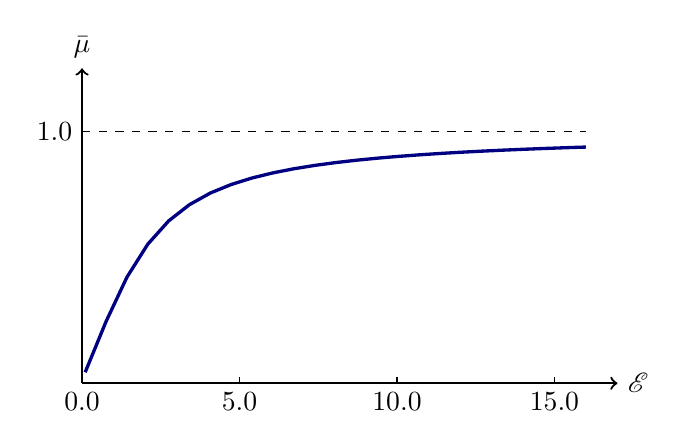
\begin{tikzpicture}[scale=0.4]
  \draw[->, thick] (0,0) -- (17,0) node[right] {$\mathscr E$};
  \draw[->, thick] (0,0) -- (0,10) node[above] {$\bar \mu$};
  \draw[scale=1.0, domain=0.1:16, variable=\x, blue!50!black, very thick]
    plot ({\x}, {((1 + exp(-2*\x))/(1 - exp(-2*\x))-1/\x)*8} );
  \draw[dashed] (0.0, 8.0) -- (16.0, 8.0);
  \draw[] ( 0.0, 0.2) -- ( 0.0, 0.0) node[below] {$0.0$};
  \draw[] ( 5.0, 0.2) -- ( 5.0, 0.0) node[below] {$5.0$};
  \draw[] (10.0, 0.2) -- (10.0, 0.0) node[below] {$10.0$};
  \draw[] (15.0, 0.2) -- (15.0, 0.0) node[below] {$15.0$};
  \draw[] ( 0.2, 8.0) -- ( 0.0, 8.0) node[left] {$1.0$};
\end{tikzpicture}
\end{figure}

\end{solution}

\subsection{Problem 2-17}

\begin{problem}
In Chapter 14 we shall derive an \emph{approximate}
partition function for a dense gas,
which is of the form
$$
  Q(N, V, T)
  =
  \frac{1}{N!}
  \left( \frac{ 2\pi m k T }{ h^2 } \right)^{3N/2}
  (V - N b)^N e^{a N^2/V k T}
$$
where $a$ and $b$ are constants that are given
in terms of molecular parameters.
%
Calculate the equation of state from this partition function.
%
What equation of state is this?
%
Calculate the thermodynamic energy and the heat capacity
and compare it to Problem 1-30.
\end{problem}

\begin{solution}
The pressure can be derived from the partition function
by Eq. \eqref{eq:pbar_from_lnQ}
%
\begin{align*}
p &=
  kT \frac{ \partial \ln Q } { \partial \, V }
=
  kT \frac{ \partial \, [ N \ln (V - N b)
   + a \, N^2 / (V k T)] }
  { \partial \, V }
\\
&=
  \frac{ N k T } { V - N b} - \frac{ a N^2 }{ V^2 }
=
  \frac{ \rho \, k T } { 1 - \rho \, b} - a \rho^2
,
\end{align*}
%
where we have introduced
the number density $\rho = N/V$ in the last step.
%
The equation of state is the van der Waals equation of states,
  [cf. Eq. (14-18) on page 304].
%
From Eqs. \eqref{eq:Ebar_from_lnQ} and \eqref{eq:S_from_lnQ},
we get
\begin{align*}
\overline E
&=
    kT^2 \left(
      \frac{ \partial \ln Q }
           { \partial T }
    \right)_{N, V}
=
  \frac{ 3 N k T }{2}
  -\frac{ a N^2 } { V}
,
\\
S
&=
    kT \left(
      \frac{ \partial \ln Q }
           { \partial T }
    \right)_{N, V}
    + k \ln Q
=
  \frac{ \overline E } { T }
  + k \ln Q
,
\\
C_V
&=
\frac{ T \partial S } { \partial T }
=
\frac{ \partial \overline E } { \partial T }
= \frac{ 3 N k}{2}
.
\end{align*}
\end{solution}

\section{Lecture 8: The Canonical Ensemble}

\subsection{Problem 3-4}

\begin{problem}
  Sate and use Euler's theorem to show
  \begin{equation}
  p
  = kT \left(
    \frac{ \partial \ln \Xi } { \partial \, V }
    \right)_{\mu, T}
  = kT \left(
    \frac{ \ln \Xi } { V }
    \right)_{\mu, T}
  .
    \label{eq:pV_lnXi}
  \end{equation}
\end{problem}

\begin{solution}
We can use the first law for the grand canonical ensemble
$$
d\ln\Xi = -\overline E \, d\beta + \beta \, p \, d V + N \, d(\beta\mu).
$$
Here $\beta$ and $\beta\,\mu$
are intensive quantities, and $V$ is extensive.
%
The first equality of Eq. \eqref{eq:pV_lnXi}
follows directly from the first law.
%
Now $\ln\Xi$, representing some free energy,
should be extensive,
and hence be a homogeneous function of order $1$
for $V$.
%
Then, Euler's theorem (page 18) says that
$$
\ln\Xi = V \, \frac{ \partial \ln \Xi } { \partial V },
$$
which is the second equality of Eq. \eqref{eq:pV_lnXi}.
\end{solution}

\subsection{Problem 3-6}

\begin{problem}
  Derive the principle thermodynamic connection formulas
  of the grand canonical ensemble starting from
  \begin{equation}
    pV = kT \ln \Xi
    \label{eq:pV_lnXi1}
  \end{equation}
  and
  \begin{equation}
    d(pV) = S \, dT + N \, d\mu + p \, dV
    \label{eq:dpV}
  \end{equation}
\end{problem}

\begin{solution}
  We start by differentiating Eq. \eqref{eq:pV_lnXi1}
  $$
  d(\ln \Xi) = d(\beta \, p V)
  = p V \, d\beta + \beta \, d(p V).
  $$
  Then, by using Eq. \eqref{eq:dpV}, we get
  \begin{align*}
    d(\ln \Xi)
    &=
    p V \, d\beta +
    \beta \, (S \, dT + N \, d\mu + p \, dV)
    \\
    &=
    \left( pV-TS \right) \, d\beta
    + N \, \beta \, d\mu + \beta p \, dV
    \\
    &=
    \left(pV-TS - N \, \mu\right) \, d\beta
    + N \, d(\beta \, \mu) + \beta p \, dV
    \\
    &=-E\, d\beta + N \, d(\beta \, \mu) + \beta p \, dV
    .
  \end{align*}
  The final step follows from Euler's theorem,
  (cf. the note).
  Thus,
  \begin{align*}
    E
    &=
    -\frac{\partial \ln \Xi } { \partial \, \beta},
    \\
    N
    &=
    \frac{\partial \ln \Xi } { \partial \, (\beta \, \mu) },
    \\
    \beta \, p
    &=
    \frac{\partial \ln \Xi } { \partial \, V }.
  \end{align*}

\paragraph*{Note on Euler's theorem.}

For a single-component system, we have
the following useful equation
\begin{equation}
  E = T \, S - p \, V + \mu \, N.
\label{eq:Euler}
\end{equation}
%
We can show this from McQuarrie's Eq. (1-60),
$$
G = \sum_i \mu_i \, N_i
$$
But by definition $G = E - TS + pV$, so
%
$$
  E = T \, S - p \, V + \sum_i \mu_i \, N_i.
$$
%
The one-component case gives Eq. \eqref{eq:Euler}.
\end{solution}

\section{Lecture 9: Grand Canonical Ensemble}

\subsection{Problem 3-15}

\begin{problem}
  Fluctuation theory provides a simple method
  to determine the characteristic function
  associated with a particular partition function.
  %
  Consider the canonical partition function
  $$
  Q(N, V, T) = \sum_E \Omega(N, V, E) \, e^{-E/kT}
  $$
  According to the theory of fluctuations,
  there is effectively only one term in this summation,
  and so we write
  $$
  Q(N, V, T) = \Omega(N, V, \overline E) \, e^{-\overline E/kT}
  $$
  Remembering that $S = k \, \ln \Omega$,
  we have, upon taking logarithms, that
  $$
  \ln Q = \frac{S}{k} - \frac{E}{kT}
  $$
  or that
  $$
  \ln Q = \frac{-A}{kT}
  $$
  Proceeding in a like manner, determine the characteristic
  thermodynamic function of the following partition functions:
  \begin{align*}
    \Xi(V, T, \mu)
    &=
    \sum_{N} Q(N, V, T) \, e^{\beta \, \mu \, N}
    \\
    \Delta(p, T, N)
    &=
    \sum_{V} Q(N, V, T) \, e^{-\beta \, p \, V}
    \\
    \phi(V, E, \beta\mu)
    &=
    \sum_{N} \Omega(N, V, E) \, e^{\beta \, \mu \, N}
    \\
    \Psi(V, T, \mu_1, N_2)
    &=
    \sum_{N_1} Q(N_1, N_2, T, V) \, e^{\beta \, \mu_1 \, N_1}
    \\
    W(p, \gamma, T, N)
    &=
    \sum_V \sum_{\mathscr A}
      Q(N, V, \mathscr A, T) \,
      e^{-\beta \, p \, V} e^{\beta \, \gamma \, \mathscr A}
  \end{align*}
  where $\mathscr A$ is surface area, and $\gamma$ is the surface tension.
\end{problem}

\begin{solution}
  For $\ln \Xi$, we have
  \begin{align*}
    \ln\Xi
    &=
    \ln Q + \beta \, \mu \, N
    =
    \frac{ -A + \mu \, N } { k T}
    =
    \frac{ p V } { kT},
  \end{align*}
  where the last step follows from Euler's theorem,
  Eq. \eqref{eq:Euler},
  $A = E - TS = -pV + \mu N$.

  Similarly,
  \begin{align*}
    \ln\Delta
    &=
    \ln Q - \beta \, p \, V
    =
    \frac{ -A - p V } { kT}
    =
    -\frac{ \mu N } { kT}
    ,
    \\
    \ln\phi
    &=
    \ln \Omega + \beta \, \mu \, N
    =
    \frac{ T S + \mu N } { kT}
    =
    \frac{ E + p V } { kT}
    =
    \frac{ H_\mathrm{enthalpy} } { k \, T }
    ,
    \\
    \ln\Psi
    &=
    \ln Q + \beta \, \mu_1 \, N_1
    =
    \frac{ -A + \mu_1 \, N_1 } { kT}
    =
    \frac{ pV - \mu_2 \, N_2 } { kT}
    ,
    \\
    \ln W
    &=
    \ln Q - \beta \, p \, V + \beta \, \gamma \, \mathscr A
    =
    \frac{ -A - p \, V + \gamma \, \mathscr A } { kT}
    =
    \frac{ - \mu N } {kT}.
  \end{align*}
\end{solution}

\subsection{Problem 3-17}

\begin{problem}
  Show that
  $$
  \overline{ (E - \overline E)^3 }
  =
  k^2\left\{
    T^4\left(
      \frac{ \partial C_V } { \partial T }
    \right)
    +
    2T^3 \, C_V
  \right\}
  $$
  and that
  $$
  \frac{
    \overline{ (E - \overline E)^3 }
  }{
    \overline E^3
  }
  =
  \mathcal O(N^{-2})
  $$
\end{problem}

\begin{solution}
  The variance of the energy distribution is
  \begin{align*}
    \sigma_E^2
    =
    \sum_j
    (E_j - \overline E)^2
    P_j
    =
    \sum_j
    (E_j - \overline E)^2
    \frac{ e^{-\beta E_j} } { Q(\beta) }
    .
  \end{align*}
  If we differentiate the expression with respect to $\beta$,
  and use $\partial \ln Q/\partial \beta = -\overline E$,
  we get
  \begin{align*}
    \frac{ \partial \sigma_E^2 }
    { \partial \beta }
    &=
    \sum_j
    (E - \overline E)^2
    (-E + \overline E)
    \frac{ e^{-\beta E_j} } { Q(\beta) }
    \\
    &=
    -\sum_j
    (E - \overline E)^3 P_j
    =
    -\overline{ (E - \overline E)^3 }
    .
  \end{align*}
  From Eq. (3-42), we get
  $$
    \frac{ \partial \left( \sigma_E^2 \right) } { \partial \beta }
    = kT^2 \, C_V,
  $$
  then
  \begin{align*}
    \overline{ (E - \overline E)^3 }
    &=
    k T^2
    \frac{ \partial ( \sigma_E^2 ) }
    { \partial T }
    =
    k T^2
    \frac{ \partial ( k T^2 C_V ) }
    { \partial T }
    \\
    &=
    k^2 T^2
    \left(
    T^2
    \frac{ \partial C_V }
    { \partial T }
    +
    2 \, T \, C_V
    \right),
  \end{align*}
  which is the desired result.

  Since $C_V \sim \mathcal O(N)$
  and $T \sim \mathcal O(1)$,
  $\overline{ (E - \overline E)^3 } \sim \mathcal O(N)$,
  and
  $$
  \frac{
    \overline{ (E - \overline E)^3 }
  }{
    \overline E^3
  }
  \sim
  \frac{ \mathcal O(N) } { \mathcal O(N^3) }
  \sim
  \mathcal O(N^{-2}).
  $$
\end{solution}

\subsection{Problem 3-24}

\begin{problem}
  Show that
  $$
  \overline{ H^2 } - \overline H^2
  =
  kT^2 C_p
  $$
  in an $N$, $p$, $T$ ensemble.
\end{problem}

\begin{solution}
  The ensemble we will use is the isothermal-isobaric ensemble,
  whose partition function is
  \begin{align}
    \Delta(p, \beta, N)
    &=
    \sum_V Q(N, V, T) \, e^{-\beta \, p \, V}
    \notag
    \\
    &=
    \sum_V \sum_E \Omega(N, V, E) \,
    e^{-\beta \, E } e^{-\beta \, p \, V}
    .
    \label{eq:Delta_def}
  \end{align}
  %

  Differentiating Eq. \eqref{eq:Delta_def}
  under fixed $N$,
  \begin{equation}
    d\ln\Delta
    =
    -\overline{H} \, d\beta
    -\beta \, \overline{V} \, dp.
    \label{eq:firstlawlnDelta}
  \end{equation}
  Then
  $$
  \overline H
  =
  -\frac{ \partial \ln \Delta } { \partial \beta }
  =
  \sum_{V}\sum_{E} H \,
  \frac{ \Omega(N, V, E) \, e^{-\beta \, H} } { \Delta(p, \beta, N) }.
  $$
  Differentiating this expression with respect to $\beta$,
  \begin{align*}
  \frac{ \partial \overline H } { \partial \beta }
  &=
  -\sum_{V}\sum_{E} H \, (H - \overline H) \,
  \frac{ \Omega(N, V, E) \, e^{-\beta \, H} } { \Delta(p, \beta, N) }.
  \\
  &=
  -\left(
  \overline{ H^2 } - \overline H^2 \right).
  \end{align*}

  We next try to establish a thermodynamic connection.
  %
  %From Problem 3-15, we know that
  %$\ln \Delta$ can be mapped to
  %$-\beta(A+pV) = \beta \, H - (S/k)$,
  %with $H = E + pV$ being the enthalpy.
  %
  Using the first law, we have
  \begin{align*}
  d(-\beta\,A)
  %&=
  %  d\left(\frac{S}{k}-\beta \, E\right)
  %=
  %\frac{dS}{k}
  %-\beta \, dE
  %-E \,d\beta
  %\\
  &=
  -E\, d\beta
  +\beta \, p \, dV+ \beta \mu dN
  \\
  d(-\beta \, A) - d(\beta \, pV)
  &=
  -E\, d\beta
  -V d( \beta \, p)
  + \beta \mu dN
  \\
  &=  -H\, d\beta
  -\beta \, V \, d p
  + \beta \mu dN.
  \end{align*}
  %
  Comparing this to Eq. \eqref{eq:firstlawlnDelta},
  we found that
  the enthalpy, $H$, in thermodynamics
  is mapped to the mean enthalpy, $\overline H$,
  and
  $$
  \ln \Delta = -\beta(A+pV) = \frac{S}{k} -\beta \, H.
  $$
  This also means that
  the entropy can be found from
  $$
  S/k = \beta \overline H + \ln \Delta,
  $$
  and
  $$
  \left(
  \frac{ \partial (S/k) }
       { \partial \beta } \right)_p
  =
  \left(
  \frac{ \partial (\beta \overline H) }
       { \partial \beta } \right)_p
  -
  \left(
  \frac{ \partial \ln \Delta }
       { \partial \beta } \right)_p
  =
  \beta
  \left(
    \frac{ \partial \overline H } { \partial \beta }
  \right)_p.
  $$
  Thus
  \begin{align*}
    \left(
      \frac{ \partial \overline H } { \partial \beta }
    \right)_p
    =
    T \left( \frac{ \partial S } { \partial \beta } \right)_p
    =
    -
    kT^3 \left( \frac{ \partial S } { \partial T} \right)_p
    =
    -kT^2 C_p.
  \end{align*}

\end{solution}

\section{Lecture 10: Fluctuations}

\subsection{Problem 3-22}

\begin{problem}
Show that the fluctuation in energy in a grand canonical ensemble is
$$
\sigma_E^2 = k \, T^2 \, C_V
  + \left( \frac{\partial \overline E } { \partial \overline N} \right)_{T, V} \sigma_N^2
$$
\end{problem}

\paragraph*{Interpretations.}

There is probably a typo here, since the units do not match.
%
The most likely fix is
\begin{equation}
  \sigma_E^2 = k \, T^2 \, C_V
  + \left( \frac{\partial \overline E }
                { \partial \overline N} \right)_{T, V}
    \sigma_N^2 \, \textcolor{red}{\times \mu}
  \label{eq:prob3-22a}
\end{equation}
%
Another possible fix is
%
\begin{equation}
  \sigma_E^2 = k \, T^2 \, C_{V,\textcolor{blue}{N}}
  + \left( \frac{\partial \overline E }
                { \partial \overline N} \right)_{T, V}^{\textcolor{blue}{2}}
    \sigma_N^2
  \label{eq:prob3-22b}
\end{equation}
%
In the second correction,
$C_V$ is interpreted as the heat capacity in the canonical ensemble,
so it is less likely.

\begin{solution}
We will show Eq. \eqref{eq:prob3-22a} first.
The partition function of the grand canonical ensemble, $\Xi$,
is defined as a superposition of
the partition functions of the canonical ensemble, $Q(N, V, T)$
at various numbers of particles, $N$:
%
\begin{align}
\Xi
  &=
  \sum_{N} Q(N, V, T) \, z^N
  \notag \\
  &=
  \sum_{N, E} \Omega(N, V, E) \, e^{-\beta \, E + \mu^* \, N}
,
  \label{eq:Xi_def}
\end{align}
%
where we have defined the reduced chemical potential $\mu^* = \beta \, \mu = \ln z$.
%
As $\ln \Omega$ corresponds to the entropy $S/k$,
$\ln Q$ corresponds to the Helmholtz free energy $S/k - \beta \, E = -\beta \, A$,
the free energy corresponding to $\ln \Xi$
is the so-called grand potential:
%
\begin{equation}
  \ln \Xi
  = \frac{S}{k} - \beta \, E + \mu^* N
  = \beta \, p \, V
  .
  \label{eq:lnXi}
\end{equation}
Here, the last step follows from Euler's theorem,
$E = T \, S - p \, V + \mu \, N$ [cf. Eq. \eqref{eq:Euler}].
%
By differentiating Eq. \eqref{eq:Xi_def}, we get
%
\begin{align*}
  \frac{ \partial \Xi } { \partial \beta }
  &=
  \sum_{N, E} \Omega(N, V, E) \cdot (-E) \cdot e^{-\beta \, E + \mu^* N}
  \\
  &=
  -\Xi \,
  \sum_{N, E} E \cdot \frac{ \Omega(N, V, E) \, e^{-\beta \, E + \mu^* N} } { \Xi }
  \\
  &=
  -\Xi \times \overline{E}
  ,
\end{align*}
%
where we have collected
$\Omega(N, V, E) \, e^{-\beta \, E + \mu^* N}/\Xi$
as the joint distribution of $E$ and $N$
in the grand canonical ensemble.
%
Dividing both sides by $-\Xi$,
we get
\begin{align}
  \overline E
  &=
  -\frac{ \partial \Xi } { \Xi \, \partial \beta }
  =
  -\frac{ \partial \ln \Xi } { \partial \beta }
  ,
  \label{eq:dXidbeta}
\end{align}
Similarly, by differentiating Eq. \eqref{eq:Xi_def}
with respect to $\mu^*$, we get
\begin{align}
  \overline N &= \frac{ \partial \ln \Xi } { \partial \mu^* }
  .
  \label{eq:dXidmu}
\end{align}
%
Combining the above two results, we get
\begin{equation}
  d \ln \Xi
  =
  \frac{ \partial \ln \Xi } { \partial \beta } d\beta
  +
  \frac{ \partial \ln \Xi } { \partial \mu^* } d\mu^*
  = -\overline E \, d\beta + \overline N \, d\mu^*
  .
  \label{eq:firstlawXi}
\end{equation}
%
We can compare this to the first law of thermodynamics,
%
\begin{align}
  dE
  &= T \, dS - p \, dV + \mu \, dN
  ,
  \notag
  \\
  d\left(\frac{S}{k} \right)
  &= \beta \, dE + \beta \, p \, dV - \mu^* \, dN
  ,
  \notag
  \\
  d\left(\frac{S}{k} - \beta \, E \right)
  &= -E \, d\beta + \beta \, p \, dV - \mu^* \, dN
  ,
  \label{eq:firstlaw_bVN}
  \\
  d\left(\frac{S}{k} - \beta \, E + \mu^* N \right)
  &= -E \, d\beta + \beta \, p \, dV + N \, d\mu^*
  .
  \notag
\end{align}
%
By Eq. \eqref{eq:lnXi},
we recognize the last expression
is the differential of $\ln \Xi$,
and with a fixed volume, $V$
it becomes
%
\begin{equation}
  d\ln \Xi = -E \, d\beta + N \, d\mu^*
  .
  \label{eq:firstlawXi2}
\end{equation}
%
Thus, to make the statistical mechanical expression, Eq. \eqref{eq:firstlawXi},
agree with the thermodynamical expression, Eq. \eqref{eq:firstlawXi2},
we should interpret $E$ and $N$ in the latter
as the ensemble averages, $\overline E$ and $\overline N$, respectively.
%
We can further differentiate
Eqs. \eqref{eq:dXidbeta} and \eqref{eq:dXidmu}
to get fluctuations of $E$ and $N$:
%
\begin{align}
  \sigma_E^2
  &=
  -\left( \frac{ \partial \overline E } { \partial \beta } \right)_{\mu^*, V}
  = \frac{ \partial^2 \ln \Xi } { \partial \beta^2 }
  ,
  \label{eq:varE}
  \\
  \sigma_N^2
  &= \left( \frac{ \partial \overline N } { \partial \mu^* } \right)_{\beta, V}
  = \frac{ \partial^2 \ln \Xi } { \partial \mu^{*2} }
  \tag{3-50}
  \label{eq:varN}
  ,
  \\
  \left( \frac{ \partial \overline E } { \partial \mu^* } \right)_{\beta, V}
  &= -\frac{ \partial^2 \ln \Xi } { \partial \mu^* \, \partial \beta }
  = - \left( \frac{ \partial \overline N } { \partial \beta } \right)_{\mu^*, V}
  \label{eq:covEN}
  .
\end{align}
The derivation of Eq. \eqref{eq:varE}
is similart to that for Eq. (3-41) in the textbook;
The derivation for Eq. \eqref{eq:varN}
is on page 61 of the textbook.

Now the heat capacity in the grand canonical ensemble can be defined as
%
\begin{align}
C_V
&= \left( \frac{ T \, \partial S } { \partial T } \right)_{\mu^*, V}
\notag \\
&= -\beta \left( \frac{ \partial S } { \partial \beta } \right)_{\mu^*, V}
= -\frac{1}{T} \left( \frac{ \partial (S/k) } { \partial \beta } \right)_{\mu^*, V}.
\label{eq:CV_def}
\end{align}
%
Using Eq. \eqref{eq:lnXi}, we have
\begin{align}
-T \, C_V
  &= \left( \frac{ \partial (\ln \Xi + \beta \, \overline E - \mu^* \, \overline N) }
  { \partial \beta } \right)_{\mu^*, V}.
  \notag
  \\
  &= \frac{ \partial \ln \Xi } { \partial \beta }
  + \overline E
  + \beta \left( \frac{ \partial \overline E } { \partial \beta } \right)_{\mu^*, V}
  - \mu^* \left( \frac{ \partial \overline N } { \partial \beta } \right)_{\mu^*, V}
  \notag
  \\
  &=
  - \beta \, \sigma_E^2
  + \mu^* \left( \frac{ \partial \overline E } { \partial \mu^* } \right)_{\beta, V}
  ,
  \notag
\end{align}
%
where we have used Eqs. \eqref{eq:dXidbeta}, \eqref{eq:varE}, and \eqref{eq:covEN}
in the last step.
%
Further using Eq. \eqref{eq:varN}, we have
\begin{equation}
T \, C_V
=
\beta \, \sigma_E^2
-
\mu^* \,
\frac{ \left( \partial \overline E / \partial \mu^* \right)_{\beta, V} }
     { \left( \partial \overline N / \partial \mu^* \right)_{\beta, V} }
\, \sigma_N^2
.
\label{eq:TCV}
\end{equation}
%
Finally, if we interpret
$$
\frac{ \left( \partial \overline E / \partial \mu^* \right)_{\beta, V} }
     { \left( \partial \overline N / \partial \mu^* \right)_{\beta, V} }
\to
\left(
  \frac{ \partial \overline E }
       { \partial \overline N }
\right)_{T, V}
,
$$
and multiply both sides of Eq. \eqref{eq:TCV} by $k T = 1/\beta$,
we recover Eq. \eqref{eq:prob3-22a}.

\paragraph*{Example on the monatomic ideal gas.}

On the monatomic ideal gas, we have
\begin{align*}
  \ln \Xi
  &= \frac{ V } { \Lambda^3 } e^{\mu^*}
  = \frac{ V (2 \, \pi \, m)^{3/2}} { h^3 } e^{\mu^*} \beta^{-3/2}
  \equiv C \, e^{\mu^*} \beta^{-3/2}
  ,
\end{align*}
where we have defind $C = V (2 \, \pi \, m)^{3/2}/h^3$.
%
Taking derivatives, we get
\begin{align*}
  \overline{ E }
  &= - \frac{ \partial \ln \Xi } { \partial \beta }
  = \frac{3}{2} C \, e^{\mu^*} \beta^{-5/2}
  ,
  \\
  \overline{ N }
  &= \frac{ \partial \ln \Xi } { \partial \mu^* }
  = C \, e^{\mu^*} \beta^{-3/2}
  ,
  \\
  \frac{ d\overline E } { d\overline N}
  &=
  \frac{3}{2\,\beta}
  ,
  \\
  \sigma_E^2
  &= - \frac{ \partial \overline{E} } { \partial \beta }
  = \frac{15}{4} \, C \, e^{\mu^*} \beta^{-7/2}
  ,
  \\
  \sigma_N^2
  &= \frac{ \partial \overline{N} } { \partial \mu^* }
  = C \, e^{\mu^*} \beta^{-3/2}
  ,
  \\
  \frac{S}{k}
  &=
  \ln \Xi + \beta \overline{E}
  -\mu^* \overline{N}
  =
  \left(\frac{5}{2} - \mu^* \right) \, C \, e^{\mu^*} \beta^{-3/2}
  ,
  \\
  \frac{C_{V, \mu^*}}{k}
  &= -\beta \left( \frac{\partial (S/k) } {\partial \beta} \right)
  = \left(\frac{15}{4} - \frac{3}{2} \, \mu^* \right)
    \, C \, e^{\mu^*} \beta^{-3/2}
  .
\end{align*}
Indeed, we have
\begin{align}
  k \, T^2 \, C_{V, \mu^*}
  =
  \sigma_E^2
  - \frac{\mu^*}{\beta} \frac{ \partial \overline E } { \partial \overline N} \sigma_N^2
  ,
\end{align}
\end{solution}


\begin{solution}[Second interpretation.]
About the second interpretation, Eq. \eqref{eq:prob3-22b},
%
Similar to Eq. \eqref{eq:CV_def},
the heat capacity in the canonical ensemble is defined as
\begin{equation}
  C_{V, N}
  = -\frac{1}{T} \left( \frac{ \partial (S/k) } { \partial \beta } \right)_{V, N}
  .
  \label{eq:CVN_def}
\end{equation}
%
To be clear, the heat capacity in the grand canonical ensemble
will be denoted as
\begin{equation}
  C_{V, \mu^*}
  = -\frac{1}{T} \left( \frac{ \partial (S/k) } { \partial \beta } \right)_{V, \mu^*}
  .
  \label{eq:CVmu_def}
\end{equation}
%
we will use the advanced technique of transforming thermodynamic variables
(i.e. chain rule),
so please ignore this section if it sounds unfamiliar.
%
We can show by the technique of determinants (see the additional notes),
or by the procedure used for solving Problem 1-28, that
\begin{align}
  \left( \frac{ \partial S } {\partial \beta } \right)_{\mu^*}
  &=
  \left( \frac{ \partial S } {\partial \beta } \right)_{N}
  -
  \frac{
    \left( \frac{ \partial \mu^* } {\partial \beta } \right)_{N}
    \left( \frac{ \partial S } {\partial N } \right)_{\beta}
  }{
    \left( \frac{ \partial \mu^* } {\partial N } \right)_{\beta}
  }
  .
  \label{eq:dSdb_muN}
\end{align}
From Eq. \eqref{eq:firstlaw_bVN}, we have
\begin{align*}
  \left( \frac{ \partial \mu^* } {\partial \beta } \right)_{N}
  &=
  \left( \frac{ \partial E } {\partial N } \right)_{\beta}
  ,
  \\
  \left( \frac{ \partial (S/k) } {\partial N } \right)_{\beta}
  &=
  \left( \frac{ \partial (\frac{S}{k} - \beta \, E) } {\partial N } \right)_{\beta}
  +
  \left( \frac{ \partial ( \beta \,  E) } {\partial N } \right)_{\beta}
  \\
  &=
  -\mu^*
  +
  \beta \, \left( \frac{ \partial E } {\partial N } \right)_{\beta}
  .
\end{align*}
Using the above two expressions, we get
\begin{align*}
  \left( \frac{ \partial S^* } {\partial \beta } \right)_{\mu^*}
  &=
  \left( \frac{ \partial S^* } {\partial \beta } \right)_{N}
  +
  \mu^* \,
  \left( \frac{ \partial E } {\partial N } \right)_{\beta}
  \left( \frac{ \partial N } {\partial \mu^* } \right)_{\beta}
  \\
  &-
  \beta \,
  \left( \frac{ \partial E } {\partial N } \right)_{\beta}^2
  \left( \frac{ \partial N } {\partial \mu^* } \right)_{\beta}
  .
\end{align*}
%
Dividing both sides by $-1/(k T) = -\beta$,
and using Eqs. \eqref{eq:CVN_def}, \eqref{eq:CVmu_def}, and \eqref{eq:varN},
we get
$$
  k T^2 C_{V, \mu^*}
  +
  \mu \,
  \left( \frac{ \partial E } {\partial N } \right)_{\beta}
  \sigma_N^2
  =
  k T^2 C_{V, N}
  +
  \left( \frac{ \partial E } {\partial N } \right)_{\beta}^2
  \sigma_N^2
  .
$$
If we interpret
$\left( \partial E / \partial N \right)_{\beta}$
as
$\left( \partial \overline E / \partial \overline N \right)_{T, V}$,
we recover Eq. \eqref{eq:prob3-22b}.
Note that we have implicitly assumed that $V$ is fixed in the above derivation.

\end{solution}


\paragraph*{Changing variables using the determinants}


We will show Eq. \eqref{eq:dSdb_muN}
using the technique of
transforming thermodynamic variables.
%
The technique is extremely useful
and it can be found in \emph{Statistical Physics}
by Landau and Lifshitz.

For two functions $f(x,y)$ and $g(x,y)$
of independent variables $x$ and $y$,
the determinant is defined as
%
\begin{equation}
\frac{ \partial (f, g) } {\partial (x, y) }
\equiv
  \left( \frac{ \partial f } {\partial x } \right)_{y}
  \left( \frac{ \partial g } {\partial y } \right)_{x}
-
  \left( \frac{ \partial f } {\partial y } \right)_{x}
  \left( \frac{ \partial g } {\partial x } \right)_{y}
.
\label{eq:det_def}
\end{equation}
%

The determinant has several useful properties.
%
First, it is antisymmetric to $f$ and $g$,
as well as to $x$ and $y$:
\begin{equation}
\frac{ \partial (f, g) } {\partial (x, y) }
=
-\frac{ \partial (g, f) } {\partial (x, y) }
=
-\frac{ \partial (f, g) } {\partial (y, x) }.
  \label{eq:det_antisym}
\end{equation}
%
If $f$ and $g$ are defined for independent variables
$u$ and $v$, which are themselves functions of $x$ and $y$,
and we want to know what $f$ and $g$ look like
if they were defined for $x$ and $y$,
then we can use the chain rule:
\begin{equation}
  \frac{ \partial (f, g) } {\partial (u, v) }
  =
  \left.
    \frac{ \partial (f, g) } {\partial (x, y) }
  \middle/
    \frac{ \partial (u, v) } {\partial (x, y) }
  \right.
  .
  \label{eq:det_ratio}
\end{equation}
%
If $f$ coincides with $x$,
or if $g$ coincides with $y$,
the determinant is reduced to a partial derivative
\begin{equation}
  \frac{ \partial (x, g) } {\partial (x, y) }
  =\left( \frac{ \partial g } {\partial y } \right)_{x}
  ,
  \qquad
  \frac{ \partial (f, y) } {\partial (x, y) }
  =\left( \frac{ \partial f } {\partial x } \right)_{y}
  ,
  \label{eq:det_parder}
\end{equation}
which can be shown directly by using Eq. \eqref{eq:det_def}.
%
In practice, we often inversely use this relation
to convert the partial derivative we want
to a determinant, and then use the other properties,
such as Eqs. \eqref{eq:det_ratio} and \eqref{eq:det_antisym},
to reach the result we want.

In our case,
we will use this technique to show Eq. \eqref{eq:dSdb_muN}.
%
We want to build a connection between
$(\partial S/\partial \beta)_{\mu^*}$
and
$(\partial S/\partial \beta)_{N}$.
Then,
\begin{align*}
  &\left( \frac{ \partial S } {\partial \beta } \right)_{\mu^*}
  =
  \frac{ \partial (S, \mu^*) } { \partial (\beta, \mu^*) }
  \\
  &=
  \left.
  \frac{ \partial (S, \mu^*) } { \partial (\beta, N) }
  \middle/
  \frac{ \partial (\beta, \mu^*) } { \partial (\beta, N) }
  \right.
  \\
  &=
  \left.
  \left[
  \left( \frac{ \partial S } {\partial \beta } \right)_{N}
  \left( \frac{ \partial \mu^* } {\partial N } \right)_{\beta}
  -
  \left( \frac{ \partial \mu^* } {\partial \beta } \right)_{N}
  \left( \frac{ \partial S } {\partial N } \right)_{\beta}
  \right]
  \middle/
  \left( \frac{ \partial \mu^* } {\partial N } \right)_{\beta}
  \right.
  \\
  &=
  \left( \frac{ \partial S } {\partial \beta } \right)_{N}
  -
  \left.
  \left( \frac{ \partial \mu^* } {\partial \beta } \right)_{N}
  \left( \frac{ \partial S } {\partial N } \right)_{\beta}
  \middle/
  \left( \frac{ \partial \mu^* } {\partial N } \right)_{\beta}
  \right.
  .
\end{align*}
Here, on the first line, we have used Eq. \eqref{eq:det_parder}
to convert the desired partial derivative,
$(\partial S/\partial \beta)_{\mu^*}$,
to a determinant.
%
On the next line, we have used Eq. \eqref{eq:det_ratio}
to change the independent variables from $\beta$ and $\mu^*$
to $\beta$ and $N$,
this will later build a connection
to the other target partial derivative,
$(\partial S/\partial \beta)_N$.
%
On the third line, we have used the definition,
Eq. \eqref{eq:det_def},
to expand the determinants on the numerator and denominator,
and for the latter,
we can use Eq. \eqref{eq:det_parder} as a shortcut.
%
The last line provides the final clean-up.

We can also show Eq. \eqref{eq:dSdb_muN}
by a procedure we used for solving Problem 1-28.
%
Similar to Eq. \eqref{eq:dSdT_pV}, we have
$$
  \left( \frac{ \partial S } {\partial \beta } \right)_{\mu^*}
  =
  \left( \frac{ \partial S } {\partial \beta } \right)_{N}
  -
  \left( \frac{ \partial S } {\partial \mu^* } \right)_{\beta}
  \left( \frac{ \partial \mu^* } {\partial \beta } \right)_{N}
  .
$$
This can be alternatively reach
with the following substitution:
$T \to \beta$, $V \to \mu^*$, and $p \to N$.
%
Then by recognizing that
$$
\left( \frac{ \partial S } { \partial \mu^* } \right)_\beta
=
\frac{
  (\partial S / \partial N)_{\beta}
} {
  (\partial \mu^* / \partial N)_{\beta}
},
$$
we also reach Eq. \eqref{eq:dSdb_muN}.


\subsection{Problem 3-23}

\begin{problem}
Show that in a two-component open, isothermal ensemble that
  \begin{align*}
    \overline{ N_1 \, N_2 }
    - \overline{N_1} \, \overline{N_2}
    &=
    kT \left(
      \frac{ \partial \overline{ N_1 } }
           { \partial \mu_2 }
      \right)_{V, T, \mu_1}
    \\
    &=
    kT \left(
      \frac{ \partial \overline{ N_2 } }
           { \partial \mu_1 }
      \right)_{V, T, \mu_2}
  \end{align*}
\end{problem}

\begin{solution}
The partition function of the grand canonical ensemble, $\Xi$,
is defined as a superposition of
the partition functions of the canonical ensemble, $Q(N_1, N_2, V, T)$
at various numbers of particles, $N_1$ and $N_2$,
of the two species:
\begin{align}
\Xi(\mu_1, \mu_2, V, T)
=
\sum_{N_1, N_2=0}^\infty
  Q(N_1, N_2, V, T) \,
  e^{\beta \, \mu_1 \, N_1 + \beta \, \mu_2 \, N_2}.
\label{eq:Xi2_def}
\end{align}
%
This means that the joint distribution of $N_1$ and $N_2$
would be given by
$$
p(N_1, N_2) = \frac{ Q(N_1, N_2, V, T) \, e^{\beta \, \mu_1 \, N_1 + \beta \, \mu_2 \, N_2} }
                   { \Xi(\mu_1, \mu_2, V, T) }.
$$
By differentiating Eq. \eqref{eq:Xi2_def},
we have
\begin{align}
  \frac{ \partial \Xi(\mu_1, \mu_2, V, T) }
       { \partial \mu_1 }
  &=
  \sum_{N_1, N_2}
    (\beta \, N_1) \times Q \cdot
    e^{\beta \, \mu_1 \, N_1 + \beta \, \mu_2 \, N_2}
  \label{eq:dXi2_dmu1a}
  \\
  &=
    \beta \, \Xi \cdot
    \sum_{N_1, N_2}
    N_1 \times p(N_1, N_2)
  \notag
  \\
  &=
    \beta \, \Xi \cdot
    \overline{ N_1 }
  .
  \label{eq:dXi2_dmu1c}
\end{align}
%
Dividing both sides by $\Xi$, we get
%
\begin{align*}
  \frac{ \partial \ln \Xi } { \partial \mu_1 }
  = \beta \cdot \overline{ N_1 },
\end{align*}
%
Similarly, we have
\begin{align}
  \frac{ \partial \ln \Xi } { \partial \mu_2 }
  = \beta \cdot \overline{ N_2 },
  \label{eq:dlnXi2_dmu2}
\end{align}
%
If we further differentiate Eq. \eqref{eq:dXi2_dmu1a}
with respect to $\mu_2$, then
\begin{align*}
  \frac{ \partial^2 \Xi(\mu_1, \mu_2, V, T) }
       { \partial \mu_1 \partial \mu_2 }
  &=
  \sum_{N_1, N_2}
    Q \cdot (\beta^2 \, N_1 \, N_2) \cdot
    e^{\beta \, \mu_1 \, N_1 + \beta \, \mu_2 \, N_2}
  \\
  &=
    \beta^2 \, \Xi \cdot
    \sum_{N_1, N_2}
    p(N_1, N_2) \cdot (N_1 \, N_2)
  \\
  &=
  \beta^2 \, \Xi \, \overline{ N_1 \, N_2 }
  .
\end{align*}
%
But if we differentiate Eq. \eqref{eq:dXi2_dmu1c}
with respect to $\mu_2$,
\begin{align*}
  \frac{ \partial^2 \Xi(\mu_1, \mu_2, V, T) }
       { \partial \mu_1 \partial \mu_2 }
  &=
    \beta \, \frac{ \partial \Xi } { \partial \mu_2 } \cdot
    \overline{ N_1 }
    +
    \beta \, \Xi \cdot
    \frac{ \partial \overline{ N_1 } } { \partial \mu_2 }
  \\
  &=
    \beta^2 \, \Xi \cdot
    \overline{ N_2 } \, \overline{ N_1 }
    +
    \beta \, \Xi \cdot
    \frac{ \partial \overline{ N_1 } } { \partial \mu_2 }
  ,
\end{align*}
%
where we have used Eq. \eqref{eq:dlnXi2_dmu2} in the second step.
To make the two expressions agree, we have
$$
  \beta^2 \, \Xi \, \overline{ N_1 \, N_2 }
  =
  \beta^2 \, \Xi \cdot
  \overline{ N_2 } \, \overline{ N_1 }
  +
  \beta \, \Xi \cdot
  \frac{ \partial \overline{ N_1 } } { \partial \mu_2 }
  ,
$$
and by eliminating $\beta^2 \, \Xi$
on both sides, we get
$$
  \overline{ N_1 \, N_2 }
  =
  \overline{ N_2 } \, \overline{ N_1 }
  +
  kT \,
  \frac{ \partial \overline{ N_1 } } { \partial \mu_2 }
  ,
$$
%
which is the desired result.
%
The second equation can be shown by swapping the indices for $1$ and $2$.
\end{solution}




\section{Lecture 11: Quantum vs. Classical Statistics}

(No problem.)

\section{Lecture 12: Ideal Monatomic Gas}

\subsection{Derive the thermodynamic potential for $(\mu, p, T)$}

\begin{problem}
Derive the thermodynamic potential for the $(\mu, p, T)$ ensemble.
\end{problem}

\begin{solution}
The answer is that no such thermodynamic potential exists.

If there were a thermodynamic potential for the $(\mu, p, T)$ ensemble,
the independent variables would be $\beta$, $\beta \, p$ and $\beta \, \mu$.
%
The partition function would look like
\begin{align*}
  \Psi
  &=
  \sum_V \Xi(N, V, \beta) \, e^{-\beta \, p \, V}
  \\
  &=
  \sum_V \sum_N Q(N, V, \beta) \, e^{\beta \, \mu \, N} \, e^{-\beta \, p \, V}
  \\
  &=
  \sum_V \sum_N \sum_E \Omega(N, V, E) \, e^{-\beta \, E}
  \, e^{\beta \, \mu \, N} \, e^{-\beta \, p \, V}
  .
\end{align*}
%
Let us now recall the process of mapping
partition functions to thermodynamic potentials.
%
For the microcanonical ensemble,
we map the logarithm of the density of states,
$\ln \Omega(N, V, E)$,
to the entropy, $S/k$.

The canonical partition function is
$Q(N, V, T) = \sum_E \Omega(N, V, E) \, e^{-\beta \, E}$,
and its logarithm corresponds to
$$
\ln Q(N, V, T) = S/k - \beta \, E = -\beta \, A,
$$
where $A = E - T \, S$ is the Helmholtz free energy.

Similarly, the partition function
of the grand canonical ensemble is
$\Xi(\mu, V, T) = \sum_N Q(N, V, T) \, e^{\beta \, \mu \, N}$,
and its logarithm corresponds to
$$
\ln \Xi(\mu, V, T) = \ln Q(N, V, T) + \beta \, \mu \, N = -\beta \, (A - \mu \, N).
$$
But from Euler's theorem, $E = T \, S - p \, V + \mu \, N$
[cf. Eq. \eqref{eq:Euler}], we know that
$$
A - \mu N = E - T S - \mu N = -p \, V,
$$
and
\begin{equation}
  \ln \Xi(\mu, V, T) = \beta \, p \, V.
\label{eq:lnXi_bpV}
\end{equation}

Finally, for our thermodynamic potential, $\Psi(\mu, V, T)$,
we would have
$$
\ln \Psi(\mu, p, T) = \ln \Xi(\mu, V, T) - \beta \, p \, V.
$$
But from Eq. \eqref{eq:lnXi_bpV},
the expression on the right-hand side is simply zero,
which means that such a thermodynamic potential
would not exist (under the above mapping to thermodynamics).
\end{solution}

\paragraph*{Another explanation.}

There is actually a simpler explanation.
%
A thermodynamic potential must be an extensive quantity,
which means that it should grow linearly with the system size.
%
But since $\mu$, $p$, and $T$ are all intensive quantities,
there is no way to specify how big the system is
and to write down the thermodynamic potential.

\paragraph*{Further discussion.}

The above argument is based on thermodynamics.
%
If we rely completely on the mathematics of statistical mechanics,
we will find that either $\ln \Psi(\mu, p, T)$
would vanish in the thermodynamic limit,
i.e. its magnitude is $\mathcal O(1)$,
or the integral for $\Psi(\mu, p, T)$ would diverge.
%
It is instructive to see this on the ideal-gas case.
%
Here, we have
\begin{align*}
  Q(N, V, T)
  &= \frac{(V/\Lambda^3)^N} {N!}, \\
  \Xi(\mu, V, T)
  &= \sum_{N=0}^\infty Q(N, V, T) \, e^{\beta \mu N}
  =
  \exp\left[
    \frac{ V \, e^{\beta \mu} } { \Lambda^3 }
  \right]
  .
\end{align*}
Then, for $\Psi(\mu, p, T)$, we have
$$
\Psi(\mu, p, T)
=\sum_{V}
  \exp\left[
    \frac{ V \, e^{\beta \mu} } { \Lambda^3 }
  \right]
  e^{-\beta \, p \, V}
\equiv
\sum_{V} e^{-\beta \, (p - p^*) \, V},
$$
where $p^* = kT \, e^{\beta \mu}/\Lambda^3$
%
Since the volume is continuous,
we should replace the sum $\sum_V \cdots$
with an integral $\int C(V) \, dV \cdots$
with some proper coefficient, $C(V)$.
%
If we assume that
$C(V)$ is a constant that does not depend on $V$,
then
\begin{align*}
\Psi(\mu, p, T)
&\propto
\int_0^\infty dV \, e^{-\beta \, (p - p^*) \, V}
\\
&=
\begin{dcases}
  \frac{1}{\beta (p - p^*)} & \mbox{if $p > p^*$} \\
  +\infty & \mbox{if $p \le p^*$},
\end{dcases}
\end{align*}
%
In the case of $p \ge p^*$,
although $\Psi(\mu, p, T)$ exists,
its magnitude is of order $\mathcal O(1)$,
i.e. $\ln \Psi(\mu, p, T)$
is not an extensive quantity,
and hence cannot represent a physical thermodynamic potential.


\subsection{Problem 5-9}

\begin{problem}
  Calculate the De Broglie wavelength of an argon atom at $25^{\circ}$C
  and compare this with the average interatomic spacing at $1$atm.
\end{problem}

\begin{solution}
The atomic weight of an Argon atom is
$39.948 \mathrm{g/mol} = 6.63352136\times 10^{-26} \mathrm{kg}$,
and the (thermal) De Broglie wavelength
\begin{align*}
\Lambda
  &= \frac{h}{ \sqrt{2\,\pi\,m_\mathrm{Ar}\,k\,T} }
  \\
  &= \frac{ 6.626070040 \times 10^{-34} }
  { \sqrt{2 \, \pi \, m_\mathrm{Ar} \cdot 1.38064852 \times 10^{-23} \cdot 298.15} }
  \\
  &\approx 1.6\times10^{-11}\mathrm{m} = 0.16\mathrm{\AA}.
\end{align*}

On the other hand,
the average interatomic spacing
  is given by $L = \sqrt[3]{V}$,
where the volume follows the ideal-gas-law $pV = kT$:
\begin{align*}
  L
  &= \left(\frac{ kT } { p} \right)^{1/3}
  = \left(
  \frac{ 1.38064852 \times 10^{-23} \cdot 298.15 }
  { 101325 } \right)^{1/3}
  \\
  &\approx 3.4\times10^{-9} \mathrm{m}
  = 34\mathrm{\AA},
\end{align*}
which is much larger than the thermal De Broglie wavelength.
%
\end{solution}

\subsection{Problem 5-14}

\begin{problem}
  Derive the standard thermodynamic formula for the entropy of mixing
  by starting with Eq. (5-20) (the Sackur-Tetrode equation):
  \begin{equation}
    S = N k \ln \left[
      \left( \frac{ 2 \, \pi \, m \, k \, T } { h^2 }
      \right)^{3/2}
      \frac{ V e^{5/2} } { N }
      \right] + S_\mathrm{elec}
    \tag{5-20}
    \label{eq:Sstd}
  \end{equation}
\end{problem}

\begin{solution}
Initially, we have two boxes of different gases
separated by a dividing partition.
%
There are $N_1$ particles of type $1$ in the first box of volume $V_1$,
and $N_2$ particles of type $2$ in the second box of volume $V_2$.
%
Upon removal of the dividing partition,
particles of either type would have volume $V = V_1 + V_2$,
and the change of entropy is given by
%
\begin{align*}
  \Delta S
  &=
    \bigl[ S(N_1, V) - S(N_1, V_1) \bigr]
  + \bigl[ S(N_2, V) - S(N_2, V_2) \bigr]
  .
\end{align*}
%
From Eq. \eqref{eq:Sstd}, we have
\begin{align}
  \Delta S
  &=
  N_1 k \ln \frac{V}{V_1}
  +
  N_2 k \ln \frac{V}{V_2}.
  \label{eq:Smix1}
\end{align}
%
If we define, for types $i = 1$ and $2$, the molar fractions
$$x_i = \frac{ N_i } { N } = \frac{ N_i } { N_1 + N_2 },$$
and assume that the volume fractions are the same
$$x_i = \frac{ V_i } { V } = \frac{ V_i } { V_1 + V_2 },$$
then Eq. \eqref{eq:Smix1} can be rewritten as
\begin{equation}
  \Delta S = -k \, N (x_1 \ln x_1 + x_2 \ln x_2),
  \label{eq:Smix}
\end{equation}
which is standard formula for the entropy of mixing.
[Cf. Terrell L. Hill,
  \emph{An Introduction to Statistical Thermodynamics},
  pages 81 and 85. ]
\end{solution}

\begin{solution}[Combinatorial solution.]
There is an combinatorial interpretation.
%
Assuming equal number densities in the two boxes,
we know that after mixing the average number of particles
in box $1$ will still be $N_1$,
but its content can be a mixture of gases of both types.
%
The initial non-mixture state corresponds to
one of the ${N \choose N_1}$ possibilities
with all type $1$ particles being in box $1$.
%
Thus, the entropy of mixing is
$$
\Delta S =  k \ln{N \choose N_1}
  = k \ln\left( \frac{ N! } { N_1! \, N_2! } \right).
$$
If we use the Stirling approximation,
$\ln N! \approx N\ln N - N$, then
\begin{align*}
  \Delta S
  &=  k (N\ln N - N_1 \ln N_1 - N_2 \ln N_2)
  \\
  &=-N_1 \ln \frac{N_1}{N} - N_2 \ln \frac{N_2}{N},
\end{align*}
which is the same as Eq. \eqref{eq:Smix}.
\end{solution}

\section{Lecture 13: Ideal Diatomic Gas}

\subsection{Problem 6-19}

\begin{problem}
Show that the thermodynamic quantities $p$ and $C_V$
are independent of the choice of a zero of energy.
\end{problem}

\begin{solution}
We start from the first law
$$dE = T \, dS - p \, dV + \mu \, dN.$$
If we understood $E$ as a function $S, V, N$,
then
$$
  dE(S, V, N)
  =
   \left( \frac{\partial E}{\partial S} \right)_{V, N} dS
  +\left( \frac{\partial E}{\partial V} \right)_{S, N} dV
  +\left( \frac{\partial E}{\partial N} \right)_{S, V} dN
  .
$$
This means
\begin{align*}
  p = -\left( \frac{\partial E}{\partial V} \right)_{S, N},
\end{align*}
and the zero of energy will not affect the pressure as its derivative.

Further, if fix the volume, $V$, and the number of particles, $N$,
then $dE = T \, dS$,
and the heat capacity
$$
  C_V \equiv \left( \frac{ T \, dS } { dT } \right)_{V, N}
  = \left( \frac{ \partial E } { \partial T } \right)_{V, N}.
$$
Again, as a derivative of the energy,
the heat capacity will not be affected by the zero of energy.
\end{solution}


\subsection{Show that when $kT \gg h\nu$, $q_\mathrm{vib} = kT/(h\nu)$.}

\begin{problem}
Show that when $kT \gg h\nu$, $q_\mathrm{vib} = kT/(h\nu)$.
\end{problem}

\begin{solution}
  (\emph{Due to Alec Fraser.})

We start from the quantum mechanical expression,
$$
q_\mathrm{vib} = \frac{e^{-\beta h\nu/2}}{1- e^{-\beta h\nu}}.
$$
Since $kT \gg h\nu$, we have $\beta h\nu \ll 1$,
which allows us to use the series expansion on $x = \beta h \nu$
around $x = 0$:
%
$$
e^x = 1 + x + \frac{x^2}{2!} + \frac{x^3}{3!} + \cdots \approx 1 + x.
$$
%
So, with $x = \beta h \nu$ and $x = \beta h \nu/2$, we get
$$
e^{-\beta h \nu} \approx 1 - \beta h \nu,
\quad
\mbox{and}
\quad
e^{-\beta h \nu/2} \approx 1 - \beta h \nu/2.
$$
Thus,
$$q_\mathrm{vib} \approx
\frac{1-\beta h\nu/2}{1- (1-\beta h\nu)}
\approx
\frac{1}{\beta h\nu} = \frac{kT}{h\nu}.
$$
\end{solution}


\section{Lecture 14: Classical Statistical Mechanics}

\subsection{Problem 7-15}

\begin{problem}
  Convert Eq. (7-40) (see Problem 7-13)
  \begin{align}
    &f(p_x, p_y, p_z) \, d p_x \, d p_y \, d p_z
    \notag \\
    &=
    (2 \pi m k T)^{-3/2}
    e^{-(p_x^2 + p_y^2 + p_z^2) / 2 m k T}
    d p_x \, d p_y \, d p_z
    \tag{7-40}
  \end{align}
  from a Cartesian coordinate to
  a spherical coordinate representation
  by writing
  \begin{align*}
    &p^2 = p_x^2 + p_y^2 + p_z^2 \\
    &p_x = p \, \cos\theta \\
    &p_y = p \, \sin\theta \, \cos\phi \\
    &p_z = p \, \sin\theta \, \sin\phi \\
    &d p_x \, d p_y \, d p_z
    \to p^2 \sin\theta d p \, d\theta \, d\phi
  \end{align*}
  and integrating over $\theta$ and $\phi$ to get
  $$
  f(p) \, dp
  =
  4 \pi (2\pi m k T)^{-3/2} p^2 e^{-p^2/2mkT} dp
  $$
  for the fraction of molecules
  with momentum between $p$ and $p+dp$.
  %
  By substituting $p = mv$,
  we get the fraction of molecules with \emph{speeds}
  between $v$ and $v+dv$:
  $$
  f(v) \, dv
  =
  4 \pi \, \left( \frac{ m } { 2 \pi k T } \right)^{3/2}
  v^2 e^{-mv^2/2kT} \, dv
  $$
\end{problem}

\begin{solution}
Conversion to the polar coordinates:
\begin{align*}
  &\int f(p_x, p_y, p_z) \, d p_x \, d p_y \, d p_z
  \\
  &=
  \int_0^\infty
    (2\pi m kT)^{-3/2} e^{-p^2/2mkT} p^2
    d p
  \int_0^\pi \sin\theta d\theta
  \int_0^{2\pi} d\phi
  \\
  &=
  \int_0^\infty
    (2\pi m kT)^{-3/2}
    p^2 e^{-p^2/2mkT}
    d p
    \int_{-1}^{1} d(\cos\theta)
    \, (2\pi)
  \\
  &=
  \int_0^\infty
    4 \, \pi (2\pi m kT)^{-3/2}
    p^2 \, e^{-p^2/2mkT}
    d p.
\end{align*}
By substituting $p = mv$, we get
\begin{align*}
  &\int_0^\infty
    4 \, \pi (2\pi m kT)^{-3/2}
    p^2 \, e^{-p^2/2mkT}
    d p
  \\
  &=
  \int_0^\infty
    4 \, \pi (2\pi m kT)^{-3/2}
    m^2 v^2 \, e^{-m v^2/2kT}
    d (m v)
  \\
  &=
  \int_0^\infty
    4 \, \pi \left(\frac{m}{2\pi kT}\right)^{3/2}
    v^2 \, e^{-m v^2/2kT}
    d v.
\end{align*}
This shows
$$
f(v) = 4 \, \pi \left(\frac{m}{2\pi kT}\right)^{3/2}
    v^2 \, e^{-m v^2/2kT}.
$$
\end{solution}

\subsection{Problem 7-16}

\begin{problem}
  Prove that the most probable molecular speed is
  $v_{mp} = (2kT/m)^{1/2}$,
  that the mean speed is
  $\langle v \rangle = (8kT/\pi m)^{1/2}$,
  and that the root-mean-square speed is
  $\langle v^2 \rangle^{1/2} = (3kT/m)^{1/2}$.
  %
  Evaluate these for $\mathrm{H}_2$ and $\mathrm{N}_2$
  at $25^{\circ}\mathrm{C}$.

  [Hint: use Problem 7-15.]
\end{problem}

\begin{solution}
The most probable speed
occurs at the zero of $f'(v) = 0$:
$$
0 =
  2 \, v \, e^{-mv^2/2kT}
  -v^2 \, \frac{mv}{kT} \, e^{-mv^2/2kT}.
$$
which shows $v_{mp} = (2kT/m)^{1/2}$.

The mean speed is
\begin{align}
  \langle v \rangle
  &=
  \int_0^\infty v \, f(v) \, dv
  =
  \frac{4 \, a^{3/2}}{\sqrt\pi}
  \int_0^\infty
    v^3 e^{-av^2} dv
  \notag
  \\
  &=
  -\frac{2 \, a^{1/2}}{\sqrt\pi}
  \int_0^\infty
    v^2 d(e^{-av^2})
  \notag
  \\
  &=
  \frac{2 \, a^{1/2}}{\sqrt\pi}
  \left(
  -\left. v^2 \, e^{-av^2} \right|_0^\infty
  +
  \int_0^\infty
    e^{-av^2} d(v^2)
  \right)
  \notag
  \\
  &=
  -\frac{2}{\sqrt{\pi a}}
  \left.  e^{-av^2}\right|_0^\infty
  =
  \frac{2}{\sqrt{\pi a}}
  =
    \sqrt{ \frac{8kT}{m} }
  .
  \label{eq:absv_ave}
\end{align}
where $a = m/(2kT)$,
and we have integrated by parts
on the third line.
%
Another way to evaluate the integral
%
\begin{align*}
  &\int_0^\infty
    v^3 e^{-av^2} \, dv
  =
  -\frac{\partial}{\partial a}
  \int_0^\infty
    v \, e^{-av^2} \, dv
  \\
  &=
  -\frac{1}{2}
  \frac{\partial}{\partial a}
  \int_0^\infty
    e^{-av^2} \, d(v^2)
  =
  -\frac{1}{2}
  \frac{\partial}{\partial a}
    \left(  \frac{1}{a} \right)
  =\frac{1}{2 \, a^2}.
\end{align*}

For the root-mean-square speed,
\begin{align}
  \langle v^2 \rangle
  &=
  \int_0^\infty v^2 \, f(v) \, dv
  =
  \frac{4 \, a^{3/2}}{\sqrt\pi}
  \int_0^\infty
    v^4 e^{-av^2} dv
  \notag \\
  &=
  \frac{4 \, a^{3/2}}{\sqrt\pi}
    \frac{ \partial^2 } { \partial a^2 }
  \int_0^\infty
    e^{-av^2} d v
  \notag \\
  &=
  \frac{4 \, a^{3/2}}{\sqrt\pi}
    \frac{ \partial^2 } { \partial a^2 }
    \left( \frac{1}{2} \sqrt{ \frac{ \pi } { a } } \right)
  =
  \frac{3}{2 \, a}
  =
  \frac{3kT}{m}
  ,
  \label{eq:v2_ave}
\end{align}
so $\langle v^2 \rangle^{1/2} = (3kT/m)^{1/2}$.
%
Another way to evaluate this:
$$
\langle v^2 \rangle
=
\langle v_x^2 + v_y^2 + v_z^2 \rangle
=
3 \langle v_x^2 \rangle
=
\frac{ 3 k T } { m },
$$
The last step is because
the distribution of $v_x$
is the Boltzmann-Maxwell distribution.

The velocities in $\mathrm{m/s}$ are listed below:
\begin{table}[h]
  \def\arraystretch{1.4}\tabcolsep=5pt
\begin{tabular}{c | c c c}
  \hline \hline
  & $v_{mp}$  & $\langle v \rangle$ & $\langle v^2 \rangle^{1/2}$\\
  \hline
  $\mathrm H_2$ &
  $1.57\times10^3$ &
  $1.77\times10^3$ &
  $1.92\times10^3$\\
  \hline
  $\mathrm N_2$ &
  $421$ &
  $475$ &
  $515$ \\
  \hline \hline
\end{tabular}
\end{table}
\end{solution}

\subsection{Problem 7-18}

\begin{problem}
  Show that the average velocity in any direction
  (say $x$, $y$, or $z$) vanishes.
  What does this mean?
\end{problem}

\begin{solution}
  [Due to Dr. Pettitt.]
  The Maxwell-Boltzmann distribution along the $x$ direction is
  $$
  f(v_x) d v_x = \sqrt{\frac{2\pi m }{kT}} e^{-m v_x^2/2kT} d v_x,
  $$
  which is a Gaussian distribution of width $\sqrt{kT/m}$
  centered at $0$.
  Thus, the mean is zero
  and the same holds for the distributions
  along the $y$ and $z$ directions.
  It means no net motion or transport in any direction.
\end{solution}

\section{Lecture 15: Classical Mechanics and Phase Space}

\subsection{Problem 7-6}

\begin{problem}
  Consider a perfect gas of molecules
  with permanent electric dipole moments $\pmb\mu$
  in an electric field $\mathscr E$.
  %
  Neglecting the polarizability fo the molecules,
  the potential energy is
  \begin{equation}
    U = -\mu \mathscr E \, \cos\theta
    \label{eq:U_muE}
  \end{equation}
  where $\theta$ is the angle between $\pmb\mu$
  and $\mathscr E$.
  %
  Using classical mechanics,
  derive an expression for the additional effect of $\mathscr E$
  on the energy $E$ and heat capacity of the gas.

  Hint: see Problem 2-16, i.e.
  $q \sim \sinh(\beta \mu \mathscr E)/(\beta \mu \mathscr E)$.
\end{problem}

\begin{solution}
Since the coupling between the electric field
and the dipole contributes $U$
to the energy function,
the relevant factor of the partition function
for the angular degrees of freedom becomes
\begin{align*}
  q_{\mathscr E}
  &=
  \int e^{-\beta U} \sin\theta d\theta \, d\phi
  =
  \int_0^\pi
  \int_0^{2\pi}
  e^{\beta \mu \mathscr E \cos\theta}
  \sin\theta \, d\theta \, d\phi
  \\
  &=
  2 \, \pi \left. \frac{
    e^{\beta \mu \mathscr E \cos\theta }
  } { \beta \mu \mathscr E}
  \right|_{0}^\pi
  =
  4 \pi \frac{ \sinh(\beta\mu\mathscr E) }
  {\beta \mu \mathscr E}
  .
\end{align*}
For the average energy we have
\begin{equation}
  \overline U
  =
  - \frac{ \partial \, \ln q_{\mathscr E} }
         { \partial \, \beta }
  =
  -\mu \mathscr E
  \left[
    \coth(\beta \, \mu \, \mathscr E)
    -
    \frac{1}{\beta \, \mu \, \mathscr E}
  \right]
  ,
  \label{eq:Uav_muE}
\end{equation}
and for the heat capacity,
  \begin{align*}
  C_V
  =-\frac{ 1 } { k T^2 }
    \frac{ \partial \overline U }
    {\partial \beta }
  =
  \frac{ \mu^2 \mathscr E^2 } { kT^2 }
  \left[
    \frac{1}{(\beta \, \mu \, \mathscr E)^2}
    -
    \frac{1}{\sinh^2(\beta \, \mu \, \mathscr E)}
  \right].
  \end{align*}

\paragraph*{Another solution.}

We can rewrite Eq. \eqref{eq:U_muE} as
a dot product
$U = -\pmb\mu \cdot \mathscr E$.
%
Then after averaging, we get
$\overline U = -\overline{ \pmb\mu} \cdot \mathscr E$.
%
But the average dipole moment, $\pmb\mu$, as a vector
is parallel to the external field, $\mathscr E$,
so
$\overline U = -\overline{ \mu} \, \mathscr E$.
If we use Eq. \eqref{eq:mubar} for $\overline\mu$,
we immediately recover Eq. \eqref{eq:Uav_muE}.
\end{solution}


\subsection{Problem 7-17}

\begin{problem}
  Show that the mean-square fluctuation of
  the velocity of the Maxwell-Boltzmann distribution
  is
  $$
  \overline{ v^2 } - \overline{v}^2
  =
  \frac{ k T } { m }
  \left(3 - \frac{8}{\pi} \right)
  $$
\end{problem}

\begin{solution}
  This follows from Eqs.
  \eqref{eq:v2_ave} and \eqref{eq:absv_ave}.
\end{solution}

\section{Lecture 16: Classical Phase Space}

\subsection{Problem 7-31}

\begin{problem}
  Let $H(p, q)$ be the classical Hamiltonian
  for a classical system of $N$ interacting particles.
  %
  Let $x_j$ be one of the $3N$ momentum components
  or one of the $3N$ spatial coordinates.
  %
  Prove the generalized equipartition theorem, namely, that
  $$
  \left\langle
    x_i \frac{ \partial H } { \partial x_j }
  \right\rangle
  = kT \, \delta_{ij}
  $$
  and from this derive the principle
  of equipartition of energy that we discussed earlier.

  Hint: Realize that the potential $U \to \infty$
  at the walls of the container.
\end{problem}

\begin{solution}
If we use $x_1, x_2, \dots$, to denote
the coordinates and momenta components,
the distribution function of the canonical ensemble
is $f(x_1, x_2, \dots) = e^{-\beta H}/Q$, and
%
\begin{align*}
  \left\langle
    x_i \frac{ \partial H } { \partial x_j }
  \right\rangle
  &=
  \frac{1}{Q} \int
    x_i \frac{ \partial H } { \partial x_j }
    e^{-\beta \, H}
    d x_1 \, d x_2 \cdots
  \\
  &=
  -
  \frac{1}{\beta}
  \frac{1}{Q}
  \int_{x_{\ne j}}
    \left(
      \int_{x_j}
      x_i \frac{ \partial \, e^{-\beta \, H} } { \partial \, x_j }
      d x_j
    \right) \, d x_{\ne j}
  \\
  &=
  \frac{1}{\beta}
  \frac{1}{Q}
  \int_{x_{\ne j}}
    \left(
      \int_{x_j}
      \frac{ \partial \, x_i } { \partial \, x_j }
      e^{-\beta \, H}
      d x_j
    \right)
  \, d x_{\ne j}
  \\
  &=
  \frac{\delta_{ij}}{\beta}
  \frac{1}{Q}
  \int e^{-\beta \, H} d x
  = kT \, \delta_{ij}
  ,
\end{align*}
%
where we have integrated by parts on the third line,
and dropped the boundary term $x_i \, e^{-\beta H}$.
This is valid because if $x_j$ is a momentum component,
it would contribute to the Hamiltonian by $x_j^2/(2m)$
and $e^{-\beta H}$ would vanish at the boundaries,
$x_j = -\infty$ and $x_j = +\infty$.
%
But if $x_j$ is a coordinate component,
we have assumed that the potential energy, $U(x_j)$,
is infinite at the two walls,
and $e^{-\beta H}$ would also vanish
at the lower and upper limits of $x_j$.
\end{solution}

\begin{problem}
  Given a potential
  $$
  U = \sum_{i=2}^\infty C_i \, q^i
  $$
  Use Problem (7-31) to derive a general
  equipartition contribution for power law potentials.
\end{problem}

\begin{solution}
Using the result of Problem 7-31, we have
$$
kT
=
\left\langle
  q \frac{ \partial U } { \partial q }
\right\rangle
=
\sum_{i = 2}^\infty
  i \, C_i \, \langle q^i \rangle
.
$$
If only a single term exists, we have
$$
  \langle U \rangle = \frac{kT}{i}.
$$
Note for odd orders, we will assume either $q \ge 0$,
or replace $q$ by $|q|$.
\end{solution}

\section{Lecture 17: Crystals, Glasses, and Polymers}

\subsection{Problem 11-11}

\begin{problem}
  Show that in a monatomic crystal the high-temperature limiting form
  of the heat capacity depends only on the existence of a cutoff frequency
  and is given by the law of Dulong and Petit.
  That is, assume only that the distribution of frequencies
  $$
  g(\nu) = 0, \qquad \mbox{for $\nu > \nu_\mathrm{max}$}
  $$
\end{problem}

\begin{solution}
  We start from
  \begin{equation}
    C_V = k
    \int_0^\infty
      \frac{ (h\nu/kT)^2 e^{-h\nu/kT} g(\nu) \, d\nu }
           { (1 - e^{-h\nu/kT})^2 }
    \tag{11-10}
  \end{equation}
  If there is a cutoff frequency, the upper limit of the integral
  can be reduced to $\nu_\mathrm{max}$, and
  at high temperature,
  we have $e^{-h\nu/kT} \approx 1 - h\nu/kT$.
  \begin{align*}
    C_V
    &= k
    \int_0^{\nu_\mathrm{max}}
      \frac{ (h\nu/kT)^2 e^{-h\nu/kT} g(\nu) \, d\nu }
           { (1 - e^{-h\nu/kT})^2 }
    \\
    &= k
    \int_0^{\nu_\mathrm{max}}
      \frac{ (h\nu/kT)^2 \cdot 1 \cdot g(\nu) \, d\nu }
           { [1 - (1-h\nu/kT))^2 }
    \\
    &= k \int_0^{\nu_\mathrm{max}} g(\nu) \, d\nu
    = 3 \, k \, N.
  \end{align*}
\end{solution}

\subsection{Entropy of a Debye crystal at low temperature}

\begin{problem}
  Show that the entropy of a Debye crystal at low
  temperature is given by
  $$
  S = \frac{4}{5} \pi^4 N k \left(\frac{kT}{h\nu_D}\right)^3
  $$
\end{problem}

\begin{solution}
  At a low temperature,
  the heat-capacity of a Debye crystal is given by
  \begin{equation}
    C_V \to \frac{ 12 \pi^4} { 5}
    N k \left( \frac{ T } { \Theta_D } \right)^3
    \tag{11-31}
  \end{equation}
  But we know that $C_V = TdS/dT$ and $S = 0$ at $T = 0$.
  So
  \begin{align*}
    S &= \int_0^T C_V(T') \frac{dT'}{T'}
    =
    \frac{ 4 \pi^4}{5}
    N k \left( \frac{T}{\Theta_D} \right)^3
    =
    \frac{ 4 \pi^4}{5}
    N k \left( \frac{k T}{h \nu_D} \right)^3
    .
  \end{align*}
  where we have used the definition
  \begin{equation}
    \Theta_D = \frac{ h \nu_D } { k}
    \tag{11-27}
  \end{equation}
  in the last step.
\end{solution}

\section{Lecture 18: Imperfect Gases}

\subsection{Problem 12-1}

\begin{problem}
  The usual form of a virial expansion is
  \begin{equation}
    \frac{pV}{RT}
    =
    1 + \frac{B(T)} {V} + \frac{C(T)}{V^2} + \cdots
    \label{eq:vir_invV}
  \end{equation}
  Some workers, however, prefer to express their data
  by expanding the compressibility factor
  in power series in the pressure
  $$
  \frac{ pV}{RT}
  =
  1+ B'(T) p + C'(T') \, p^2 + \cdots
  $$
  Find the relations between the two sets of virial coefficients.
\end{problem}

\begin{solution}
  For convenience, we will denote $P = p/RT$, $\rho = 1/V$.
  Then Eq. \eqref{eq:vir_invV} shows that
  \begin{align*}
    \rho
    &=
    \frac{ P } { 1 + B \, \rho + C \, \rho^2 + \cdots}
    \\
    &=
    \frac{ P } { 1 + B \, \frac{ P } { 1 + B \rho + \dots}
    + C \, \left( \frac{P}{1+B\,\rho+\cdots} \right)^2 + \cdots}
    .
  \end{align*}
  To the second order, we have
  \begin{align*}
    \rho
    &\approx
    \frac{ P } { 1 + B \, P}
    \approx
    P - B \, P^2
    .
  \end{align*}
  Using this in Eq. \eqref{eq:vir_invV}, we get
  \begin{align*}
  \frac{pV}{RT}
  &\approx
  1 + B (P - B P^2) + C P^2 + \cdots
  \\
  &=
  1 + B P + (C-B^2) P^2 + \cdots
  \end{align*}
  Thus,
  \begin{align*}
    B' &= \frac{B}{RT}, \\
    C' &= \frac{C - B^2}{(RT)^2}.
  \end{align*}
  For reference, we have for the next order
  $$
  D' = (D -3BC+2B^3)/(RT)^3.
  $$
\end{solution}

\begin{solution}[To higher orders.]
  Here we give a more general mathematical technique
  to extend the result to higher orders.
  %
  Then the usual form is
  $$
  P = V^{-1} \left(1 + \sum_{n=1}^\infty B_{n+1} \, V^{-n}\right),
  $$
  where $B_2 = B(T)$, $B_3 = C(T)$, \dots.
  %
  In the pressure expansion, we have
  $$
  P V = 1 + \sum_{n=1}^\infty B'_{n+1} \, p^n,
  $$
  where $B'_2 = B'(T)$, $B'_3 = C'(T)$, \dots.
  %
  For $n > 0$, we have
  %
  $$
  B'_{n+1}
  =
  \oint \frac{ P V } { p^{n+1} } \frac{d p}{2\pi i}
  =\frac{(RT)^{-n}}{2\pi i}
  \oint \frac{ V \, d P } { P^n }
  ,
  $$
  where the integral is carried around a small circle
  enclosing the origin of the complex plane.
  %
  \begin{align*}
    B'_{n+1}
    &= -\frac{(RT)^{-n}}{n-1}
    \frac{1}{2\pi i} \oint V \, d \left( \frac{ 1 } { P^{n-1} } \right)
    \\
    &= \frac{(RT)^{-n}}{n-1}
    \frac{1}{2\pi i} \oint \frac{ d V } { P^{n-1} }
    \\
    &= -\frac{(RT)^{-n}}{n-1}
    \frac{1}{2\pi i} \oint \frac{ d \rho } { P^{n-1} \rho^2 }
    \\
    &=
    -\frac{(RT)^{-n}}{n-1}
    \frac{1}{2\pi i} \oint
    \frac{ d \rho } { (1+\sum_{m=1}^\infty B_m \rho^m )^{n-1} \rho^{n+1} }
    \\
    &= -\frac{(RT)^{-n}}{(n-1)}
      \left[
        \left(1+\sum_{m=1}^\infty B_m \rho^m \right)^{1-n}
      \right]_n
    ,
  \end{align*}
  %
  where
  we have integrated by parts on the second line,
  $\bigl[ R(\rho) \bigr]_n$
  means the coefficient of $\rho^n$ of the polynomial $R(\rho)$.
  %
  The last expression is understood
  as the $n$th coefficient of the series expansion
  of $\left(1+\sum_{m=1}^\infty B_{m+1} \rho^m \right)^{1-n}$
  in $\rho$.
  %
  For example, for $n = 2$, we have
  to the leading order,
  $$
  (1 + B_2 \rho + B_3 \rho^2 + \cdots)^{-1}
  =
  1 - B_2 \rho + (B_2^2 - B_3) \rho^2 + \cdots
  $$
  and we have
  $$
  B_2' = \frac{-1}{(RT)^2} (B_2^2 - B_3)
  = \frac{ C - B^2 } { (RT)^2 }.
  $$
  And for $n = 3$, we have
  to the leading order,
  \begin{align*}
  &\left( 1 + B_2 \rho + B_3 \rho^2 + B_4 \rho^3 \cdots \right)^{-2}
  \\
  &=
  1 - 2 B_2 \rho + (2 B_2^2 - 3 B_3) \rho^2
    - 2 (B_4 - 3 B_3 B_2 + 2B_2^3) \rho^3
    + \cdots
  \end{align*}
  and we have
  $$
  B_4' = \frac{1}{(RT)^3} (B_4 - 3 B_3 B_2 + 2 B_2^3)
  = \frac{ D - 3 B C + 2 B^3 } { (RT)^3 }.
  $$
\end{solution}

\subsection{Problem 12-10}

\begin{problem}
  Show that
  $$
  B_2 =
  -\frac{1}{6kT}
  \int_0^\infty
  r \frac{ du(r) } { dr } e^{-u(r)/kT} 4 \pi r^2 \, dr
  $$
  is equivalent to
  $$
  B_2
  =
  -\frac{1}{2}
  \int_0^\infty
  (e^{-\beta u(r)} - 1)
  4 \, \pi r^2 \, dr
  $$
  State the condition on $u(r)$ that is necessary.
\end{problem}

\begin{solution}
  From the first expression, we have
  \begin{align*}
  B_2 &=
  -\frac{1}{6kT}
  \int_0^\infty
  r \frac{ du(r) } { dr } e^{-u(r)/kT} 4 \pi r^2 \, dr
  \\
    &=
  -\frac{1}{6}
  \int_0^\infty
    4 \pi r^3 \frac{ d(1- e^{-u(r)/kT}) } { dr } \, dr
  \\
  &=
  \left.
    -\frac{ 4 \pi }{6} r^3 \, (1- e^{-u(r)/kT})
  \right|_{r=0}^{\infty}
  +
  \frac{1}{2}
  \int 4 \pi r^2 \, (1- e^{-u(r)/kT}) \, dr
  ,
  \end{align*}
  where we have integrated by parts on the third line.
  If $u(r)$ tends to $0$ quicker than $1/r^3$ as $r \to \infty$
  then
  $$
  4\pi r^3 (1 - e^{-u(r)/kT}) \approx 4 \pi r^3 u(r)/kT \to 0,
  $$
  and we can drop the first expression on the right,
  and reach the second expression.
\end{solution}

\section{Lecture 19: Classical Monatomic liquids}

\subsection{Law of corresponding states}

\begin{problem}
Law of corresponding states: Take van der Waale's
equation for $n = 1$
$$
\left( p + a/V^2 \right)(V - b) = RT
$$
and write in terms of reduced variables of
the critical point $T/T_c$, $p/p_c$, $V/V_c$.
%
Substitute
  $T_c = 8a/(27bR)$
  $p_c = a/(27b^2)$,
  and
  $V_c = 3b$, 
and find the law of corresponding states for gases.
\end{problem}

\begin{solution}
  In terms of reduced variables,
  $$
  \left( p_c p^* + \frac{ a } { V_c^2 {V^*}^2 } \right)
  (V_c V^* - b) = R T_c T^*.
  $$
  With
  $T_c = 8a/(27bR)$,
  $p_c = a/(27b^2)$,
  and
  $V_c = 3 \, b$,
  $$
  \left( p^* + \frac{ 3 } { {V^*}^2 } \right)
  \left(V^* - \frac{1}{3} \right)
  = \frac{8}{3} \, T^*.
  $$
  Cf. Problem 14-1.
\end{solution}


\subsection{Problem 13-4}

\begin{problem}
  Show that the fugacity is related to the intermolecular potential by
  $$
  \ln f
  =
  \ln(\rho k T)
  +
  \frac{ \rho }{ k T }
  \int_0^\infty
  \int_0^1
  u(r) g(r, \rho, \xi) 4 \pi r^2 \, dr \, d\xi
  $$
  Using this formula, derive a virial expansion for $f$.
\end{problem}

\begin{solution}
  Fugacity is defined as
  \begin{align*}
    f = p^\mathrm{i.g.} \, e^{(\mu - \mu^\mathrm{i.g.})/kT}
      = \frac{ k T } { \Lambda^3 } e^{\beta \, \mu}.
  \end{align*}
  where $p^\mathrm{i.g.}$ and $\mu^\mathrm{i.g.}$
  are the pressure and chemical potential of
  the corresponding ideal gas, and
  in the grand canonical ensemble
  $$
  p^\mathrm{i.g.}/kT
  = \frac{1}{V} \ln \left[
    \sum_{N=0}^\infty \frac{V^N}{\Lambda^{3N}}e^{\mu^\mathrm{i.g.} N/kT}
    \right]
  = \frac{ e^{\mu^\mathrm{i.g.}/kT} }{ \Lambda^3 }.
  $$
  From Eq. (13-34), we have
  \begin{equation}
    \frac{\mu}{kT}
    =
    \ln(\rho\Lambda^3)
    +
    \frac{\rho}{kT}
    \int_0^1
    \left( \int_0^\infty
    u(r) \, g(r; \xi) 4 \pi r^2 \, dr \right) \, d\xi
    \tag{13-34}
  \end{equation}
  So
  \begin{equation*}
    \ln f
    =
    \ln(\rho kT)
    +
    \frac{\rho}{kT}
    \int_0^\infty
    \int_0^1
    u(r) \, g(r, \rho, \xi) 4 \pi r^2 \, dr \, d\xi.
  \end{equation*}

  For the virial expansion, we first expand $\ln[f/(\rho kT)]$ as
  $$
  \ln \frac{ f }{ \rho k T} = \sum_{j=1} b_j \rho^j.
  $$
  We have, similar to Eq. (13-87),
  \begin{align*}
  g(r, \rho, \xi)
    &=
    e^{-\xi u(r)/kT}
    y(r, \rho, \xi)
    \\
    &=
    e^{-\xi u(r)/kT}
    \left(
    1 + \rho g_1(r, \xi)
    + \rho^2 g_2(r, \xi) + \cdots
    \right)
    .
  \end{align*}
  Then
  \begin{align*}
    \ln \frac{ f } { \rho k T }
    &=
    \sum_{j=1}^\infty
    \rho^{j+1}
    \int_0^\infty
    \int_0^1
    \frac{u(r)} {kT} \, e^{-\xi u(r)/kT}
    g_j(r, \xi) 4 \pi r^2 \, dr \, d\xi.
  \end{align*}
  Thus,
  \begin{align*}
    b_{j+1}
    &=
    \int_0^\infty
    \int_0^1
    \frac{u(r)} {kT} \, e^{-\xi u(r)/kT}
    g_j(r, \xi) 4 \pi r^2 \, dr \, d\xi
    .
  \end{align*}

  Alternatively,
  we have
  \begin{align*}
    \ln \frac{ f } { \rho k T }
    &=
    \rho
    \int_0^\infty
    \left(
      \int_0^1
      \frac{u(r)} {kT} \, e^{-\xi u(r)/kT}
      y(r, \rho, \xi) \, d\xi \right)
     4 \pi r^2 \, dr
    \\
    &=
    \rho
    \int_0^\infty
    \left(
      \int_0^1
      \frac{ \partial (1 - e^{-\xi u(r)/kT}) } { \partial \xi }
      y(r, \rho, \xi) \, d\xi
    \right)
     4 \pi r^2 \, dr
    \\
    &=
    \rho
    \int_0^\infty
      (1 - e^{-u(r)/kT})
      y(r, \rho)
     4 \pi r^2 \, dr
    \\
    &+\rho
    \int_0^\infty
    \left(
      \int_0^1
      \frac{ \partial y(r, \rho, \xi) } { \partial \xi}
      (e^{-\xi u(r)/kT} - 1)
      \, d\xi \right)
     4 \pi r^2 \, dr
    .
  \end{align*}
  where we have integrated by parts in the last step.
  So
  \begin{align*}
    b_{j+1}
    &=
    \int_0^\infty
      g_j(r, 1) (1 - e^{-u(r)/kT})
      \, 4 \pi r^2 \, dr
    \\
    &+
    \int_0^\infty
      \left(
        \int_0^1 \frac{ \partial g_j(r, \xi) } { \partial \xi}
        (e^{-\xi u(r)/kT} - 1) \, d\xi
      \right)
    4 \pi r^2 \, dr
    .
  \end{align*}
  Once we have $b_j$'s, we can exponentiate the series
  $$
  f = \rho k T \exp\left( \sum_{j=1} b_j\rho^j \right).
  $$
\end{solution}


\subsection{Problem 13-7}

\begin{problem}
  Show that $V^n N! / N^n (N-n)!$
  can be written as $V^n[1 + \mathcal O(N^{-1})]$.
  This factor occurs in Eq. (13-9)
  \begin{align}
    g^{(n)}(\mathbf r_1, \dots, \mathbf r_n)
    &=
    \frac{ V^n N! } { N^n (N-n)! } \cdot
    \frac{
      \int\cdots\int e^{-\beta U_N} \, d\mathbf r_{n+1}\cdots d\mathbf r_N
    } { Z_N }
    \notag
    \\
    &=
    V^n(1 + \mathcal O(N^{-1}))
    \frac{
      \int\cdots\int e^{-\beta U_N} \, d\mathbf r_{n+1}\cdots d\mathbf r_N
    } { Z_N }
    \tag{13-9}
  \end{align}
  for $g^{(n)}(\mathbf r_1, \dots, \mathbf r_n)$.
  Show that this implies that
  $g^{(2)} \to 1 + \mathcal O(N^{-1})$ as $r \to \infty$.
\end{problem}

\begin{solution}
  \begin{align*}
    \frac{ N! } { N^n (N-n)! }
    &=
    \frac{ N(N-1)\cdots (N-n+1) }
      { N^n }
    \\
    &=
    \left(1 - \frac{1}{N}\right)
    \cdots
    \left(1 - \frac{n-1}{N}\right)
  \end{align*}
  Since $N \gg n$, we have
  $1/N \sim \mathcal O(N^{-1})$,
  $(n-1)/N \sim \mathcal O(N^{-1})$,
  and
  \begin{align*}
    \left(1 - \frac{1}{N}\right)
    \cdots
    \left(1 - \frac{n-1}{N}\right)
    &\approx
    1-\left(
    \frac{1}{N}
    + \cdots +
    \frac{n-1}{N}
    \right)
    \\
    &\sim
    1 + \mathcal O(N^{-1}).
  \end{align*}
  
  Using the above result for $g^{(2)}$, we have
  \begin{align*}
    g^{(2)}(\mathbf r_1, \mathbf r_2)
    =
    V^2(1 + \mathcal O(N^{-1}))
    \frac{
      \int\cdots\int e^{-\beta U_N} \, d\mathbf r_{3}\cdots d\mathbf r_N
    } { Z_N }
    .
  \end{align*}
  The integral in the above expression
  would be independent of
  $|\mathbf r_1 - \mathbf r_2| = r_{12} = r$
  for a sufficiently large distance.
  \begin{align*}
    g^{(2)}(r)
    &\approx
    (1 + \mathcal O(N^{-1}))
    \frac{\int d\mathbf r_1 \int d\mathbf r_2
      \int\cdots\int e^{-\beta U_N} \, d\mathbf r_{3}\cdots d\mathbf r_N
    } { Z_N }
    \\
    &=
    (1 + \mathcal O(N^{-1})).
  \end{align*}
\end{solution}

%\section{Lecture 20: Density Distributions and Correlation Functions}
%
%\section{Lecture 21: Evaluating Correlation Functions}
%
%\section{Lecture 22: Equilibria and Multi-Component Systems}
%
%\section{Lecture 23: Thermodynamic Perturbation Theory}
%
%\section{Lecture 24: Electrolyte Solutions}

\end{document}

